\documentclass[11pt]{article}

\usepackage[margin=2.5cm]{geometry}
\usepackage{amsmath}
\usepackage{amssymb}
\usepackage{graphicx}
\usepackage{booktabs}
\usepackage{hyperref}

\graphicspath{{../../plots/derivatives/}}

\newcommand{\Mpch}{\,h^{-1}\,\mathrm{Mpc}}
\newcommand{\xivec}{\boldsymbol{\xi}}
\newcommand{\dd}{\mathrm{d}}

\title{Technical note: Fisher-matrix forecasts from ASTRA
environment-split clustering}
\author{ASTRA clustering project}
\date{June 2026}

\begin{document}
\maketitle

\begin{abstract}
We forecast cosmological constraints on $\{\omega_b,\omega_{cdm},n_s,
\sigma_8\}$ from the redshift-space two-point clustering of an HOD galaxy
sample split by cosmic-web environment with the ASTRA classification.
Cosmology derivatives come from the AbacusSummit linear derivative grid;
covariances come from $500\Mpch$ subboxes of the fiducial box.  The note
documents the full chain of methodological refinements that the project
went through, each driven by a concrete failure of the previous step:
(i) paired central differences and the discovery that the available HOD
catalogs are \emph{not} matched across cosmologies, so the cosmology
derivatives are HOD-contaminated; (ii) phase-matched full-box differences
(Tier~0) that remove the derivative \emph{noise} but not the contamination
\emph{bias}; (iii) an explicit HOD-contamination subtraction calibrated on
extra fiducial HOD draws (Tier~1); (iv) a joint cosmology$+$HOD Fisher
that marginalises the HOD nuisances under a prior; (v) a covariance pooled
across cosmologies that lifts the Hartlap limit and lets the quadrupole
and random-quantile statistics into the data vector; and finally (vi) a
global linear response model fit across $\sim 50$ HOD draws \emph{per}
cosmology, whose cosmology derivatives are HOD-clean by construction and
which supersedes the contamination-subtraction machinery.  The headline
methodological results are that the ASTRA environment split, the
quadrupole, and the random-quantile statistics each add information beyond
the full-sample monopole even after HOD marginalisation.
\end{abstract}

\tableofcontents

\section{Fisher formalism}
\label{sec:formalism}

For a Gaussian-distributed data vector $\xivec$ with a parameter-independent
covariance $\mathsf{C}$, the Fisher information matrix for parameters
$\theta_\alpha$ is
\begin{equation}
F_{\alpha\beta} \;=\;
\frac{\partial \xivec}{\partial \theta_\alpha}^{\!\top}
\mathsf{C}^{-1}
\frac{\partial \xivec}{\partial \theta_\beta},
\qquad
\sigma(\theta_\alpha) \;=\; \big[(F^{-1})_{\alpha\alpha}\big]^{1/2}
\label{eq:fisher}
\end{equation}
\cite{tegmark1997}.  The marginalised error on $\theta_\alpha$ uses the
inverse of the \emph{full} matrix; the conditional (all other parameters
fixed) error is $F_{\alpha\alpha}^{-1/2}$.

The curves shown later are not measured posteriors but the likelihood
implied by Eq.~(\ref{eq:fisher}): the log-likelihood is expanded to second
order about the fiducial point, so it is by construction Gaussian,
\begin{equation}
\mathcal{L}(\theta) \;\propto\;
\exp\!\left[ -\tfrac{1}{2}\,(\theta-\theta_{\rm fid})^\top F\,
(\theta-\theta_{\rm fid}) \right].
\label{eq:gauss}
\end{equation}
For a parameter handled in the logarithm (e.g.\ $\ln\omega_b$) the physical
width follows from the same expansion,
$\sigma(\omega_b)=\omega_{b,{\rm fid}}\,\sigma(\ln\omega_b)$.

Our data vectors are built from the redshift-space 2PCF multipoles
($\ell=0,2$; 15 bins over $0<s<150\Mpch$) of: the full LRG-like sample;
the four ASTRA environment quantiles of the data (Q1 most underdense,
Q4 most overdense); the four quantiles of the \emph{random} catalog, which
ASTRA classifies on the same Delaunay tessellation and which therefore
trace the same cosmic web; and the cross-correlations of the full sample
with each quantile.  The measurement pipeline (Landy--Szalay estimator) is
described in the companion zero-crossing note.

The inverse covariance built from $N$ samples and $p$ bins is biased; we
apply the Hartlap correction $(N-p-2)/(N-1)$ \cite{hartlap2007} to
$\mathsf{C}^{-1}$ throughout.  This factor is what makes the number of
covariance samples the binding constraint on how long a data vector can be,
a theme that recurs below.

\section{Simulations and the HOD-mismatch problem}
\label{sec:sims}

Table~\ref{tab:cosmologies} lists the nine simulations: the fiducial
cosmology and the four $\pm$ pairs of the AbacusSummit linear derivative
grid \cite{maksimova2021}, all at phase \texttt{ph000}, $z=0.5$, each
populated with an LRG-like HOD catalog ($\sim4\times10^6$ galaxies) from
the EMC emulator set.  The grid holds the CMB acoustic scale $\theta_\ast$
fixed ($h$ retuned) and, except for the $\sigma_8$ pair, retunes $A_s$ so
$\sigma_8$ is held constant; the cosmology signal in each pair is therefore
the response to a \emph{single} parameter.

\begin{table}[ht]
\centering
\begin{tabular}{llll}
\toprule
Cosmology & Variation & Fisher HOD pick & Ensemble \\
\midrule
\texttt{c000} & fiducial (Planck 2018 $\Lambda$CDM) & \texttt{hod484} & 50 draws \\
\texttt{c100} / \texttt{c101} & $\pm 2\%$ in $\ln\omega_b$ & \texttt{hod179} / \texttt{hod152} & 50 / 50 \\
\texttt{c102} / \texttt{c103} & $\pm 3.3\%$ in $\ln\omega_{cdm}$ & \texttt{hod556} / \texttt{hod861} & 50 / 50 \\
\texttt{c104} / \texttt{c105} & $\pm 0.01$ in $n_s$ & \texttt{hod498} / \texttt{hod589} & 50 / 50 \\
\texttt{c112} / \texttt{c113} & $\pm 2\%$ in $\sigma_8$ & \texttt{hod507} / \texttt{hod483} & 50 / 50 \\
\bottomrule
\end{tabular}
\caption{Simulations of the 4-parameter $\Lambda$CDM Fisher design.  All are
AbacusSummit base boxes ($2000\Mpch$, phase \texttt{ph000}).  ``Fisher HOD
pick'' is the single catalog used for the early ($\pm$-pair) derivatives;
``Ensemble'' is the per-cosmology set of $\sim 50$ maximin-selected HOD
draws used by the global response model of Section~\ref{sec:global}.}
\label{tab:cosmologies}
\end{table}

\paragraph{The core problem.}
The emulator catalogs are \emph{not} HOD-matched across cosmologies: each
cosmology carries its own random draws from the 12-parameter yuan23 HOD
prior, with different parameter values at the same \texttt{hodNNN} index
(verified from all catalog headers; zero exact matches).  A derivative
formed from a single catalog per cosmology therefore mixes the cosmology
signal with the difference in galaxy--halo connection between the two
catalogs.  Measured directly, the \texttt{c100}$-$\texttt{c101} difference
is a scale-dependent $-6\%$ to $+9\%$ tilt of $\xi_0$, against a
$\sim 1\%$ physical $\omega_b$ signal at fixed $\sigma_8$ and
$\theta_\ast$; the $\sigma_8$ pair difference loses $\sim 89\%$ of its
amplitude to a cancelling HOD mismatch.  Removing this contamination is the
thread that connects every method below.

\section{Derivatives}
\label{sec:derivatives}

\subsection{Paired subbox central differences}

The first derivative estimator differences the \emph{same} $500\Mpch$
subbox $i$ in the two cosmologies of a pair before averaging,
\begin{equation}
\frac{\partial \xivec_i}{\partial \theta}
=
\frac{\xivec_i(\theta+\Delta\theta)-\xivec_i(\theta-\Delta\theta)}
{2\,\Delta\theta}.
\label{eq:centraldiff}
\end{equation}
Because the grid simulations share the fiducial phases and our pipelines
share random seeds, cosmic variance largely cancels in
Eq.~(\ref{eq:centraldiff}); the mean over the 64 subboxes gives the
derivative and its scatter the uncertainty.
Figure~\ref{fig:derivatives} shows these derivatives for all four
parameters and all measured statistics.

\begin{figure}[ht]
\centering
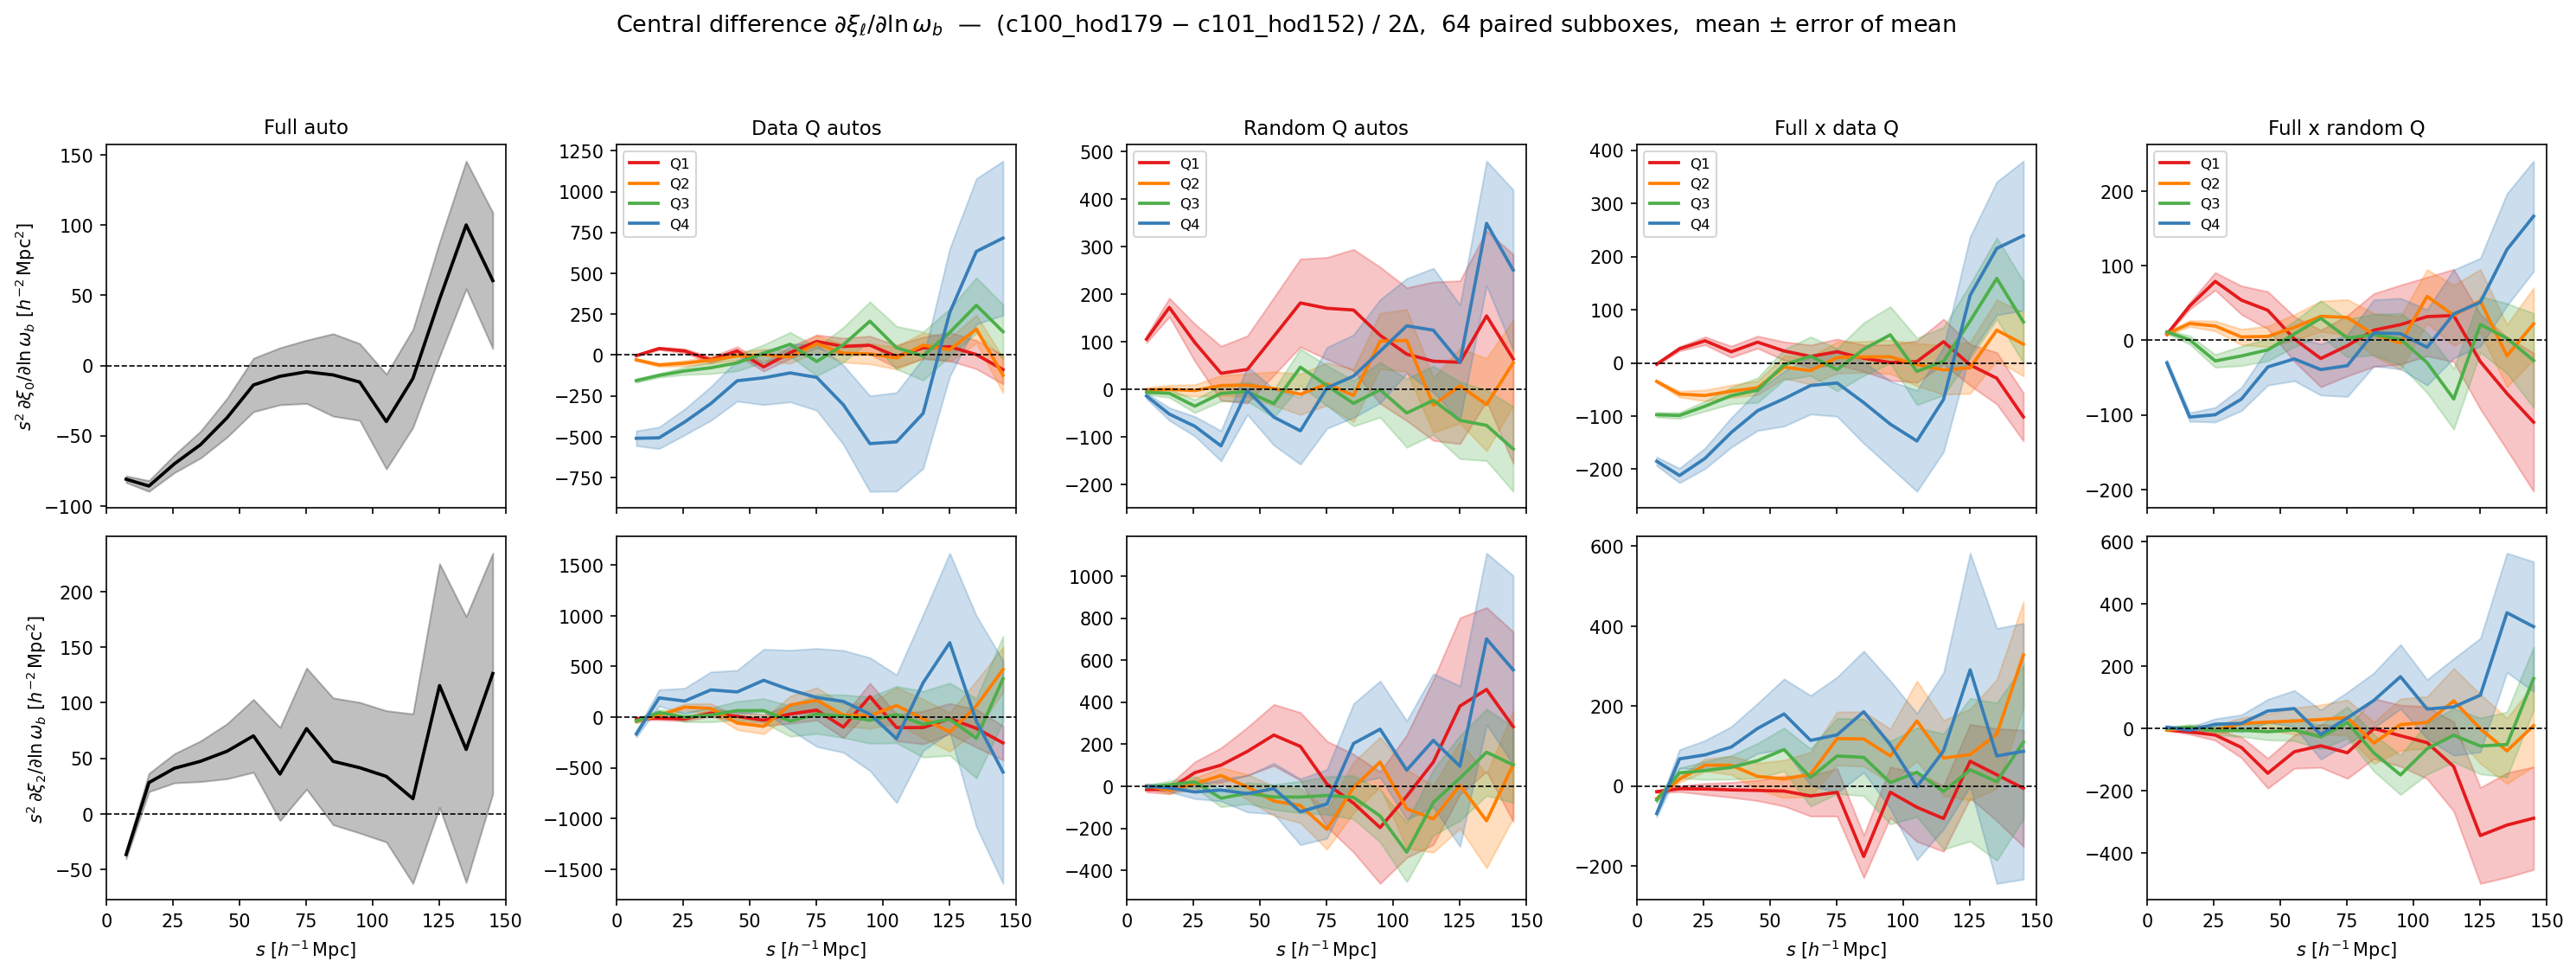
\includegraphics[width=0.49\textwidth]{derivative_lnwb.png}\hfill
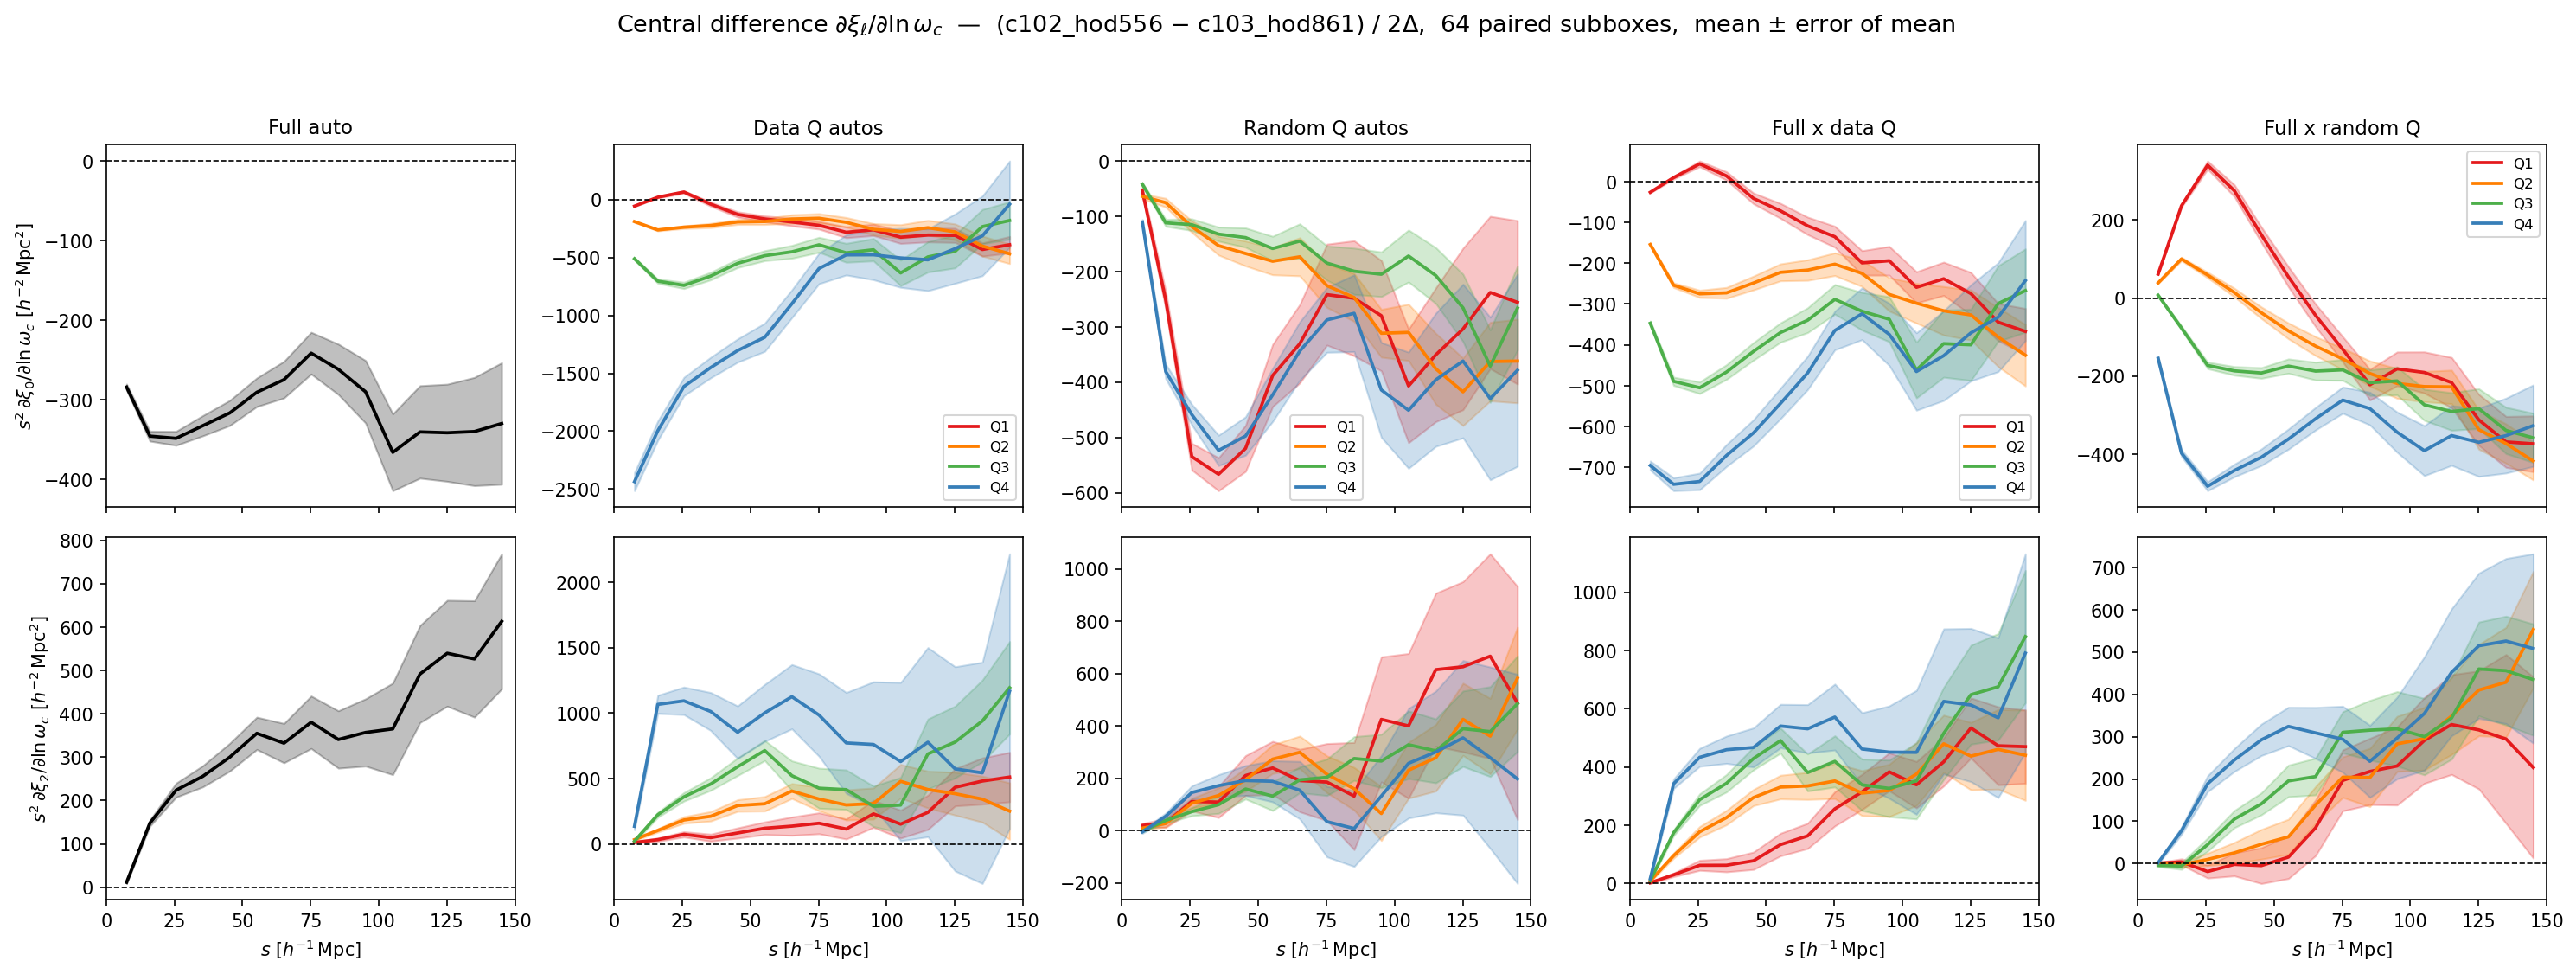
\includegraphics[width=0.49\textwidth]{derivative_lnwc.png}\\[4pt]
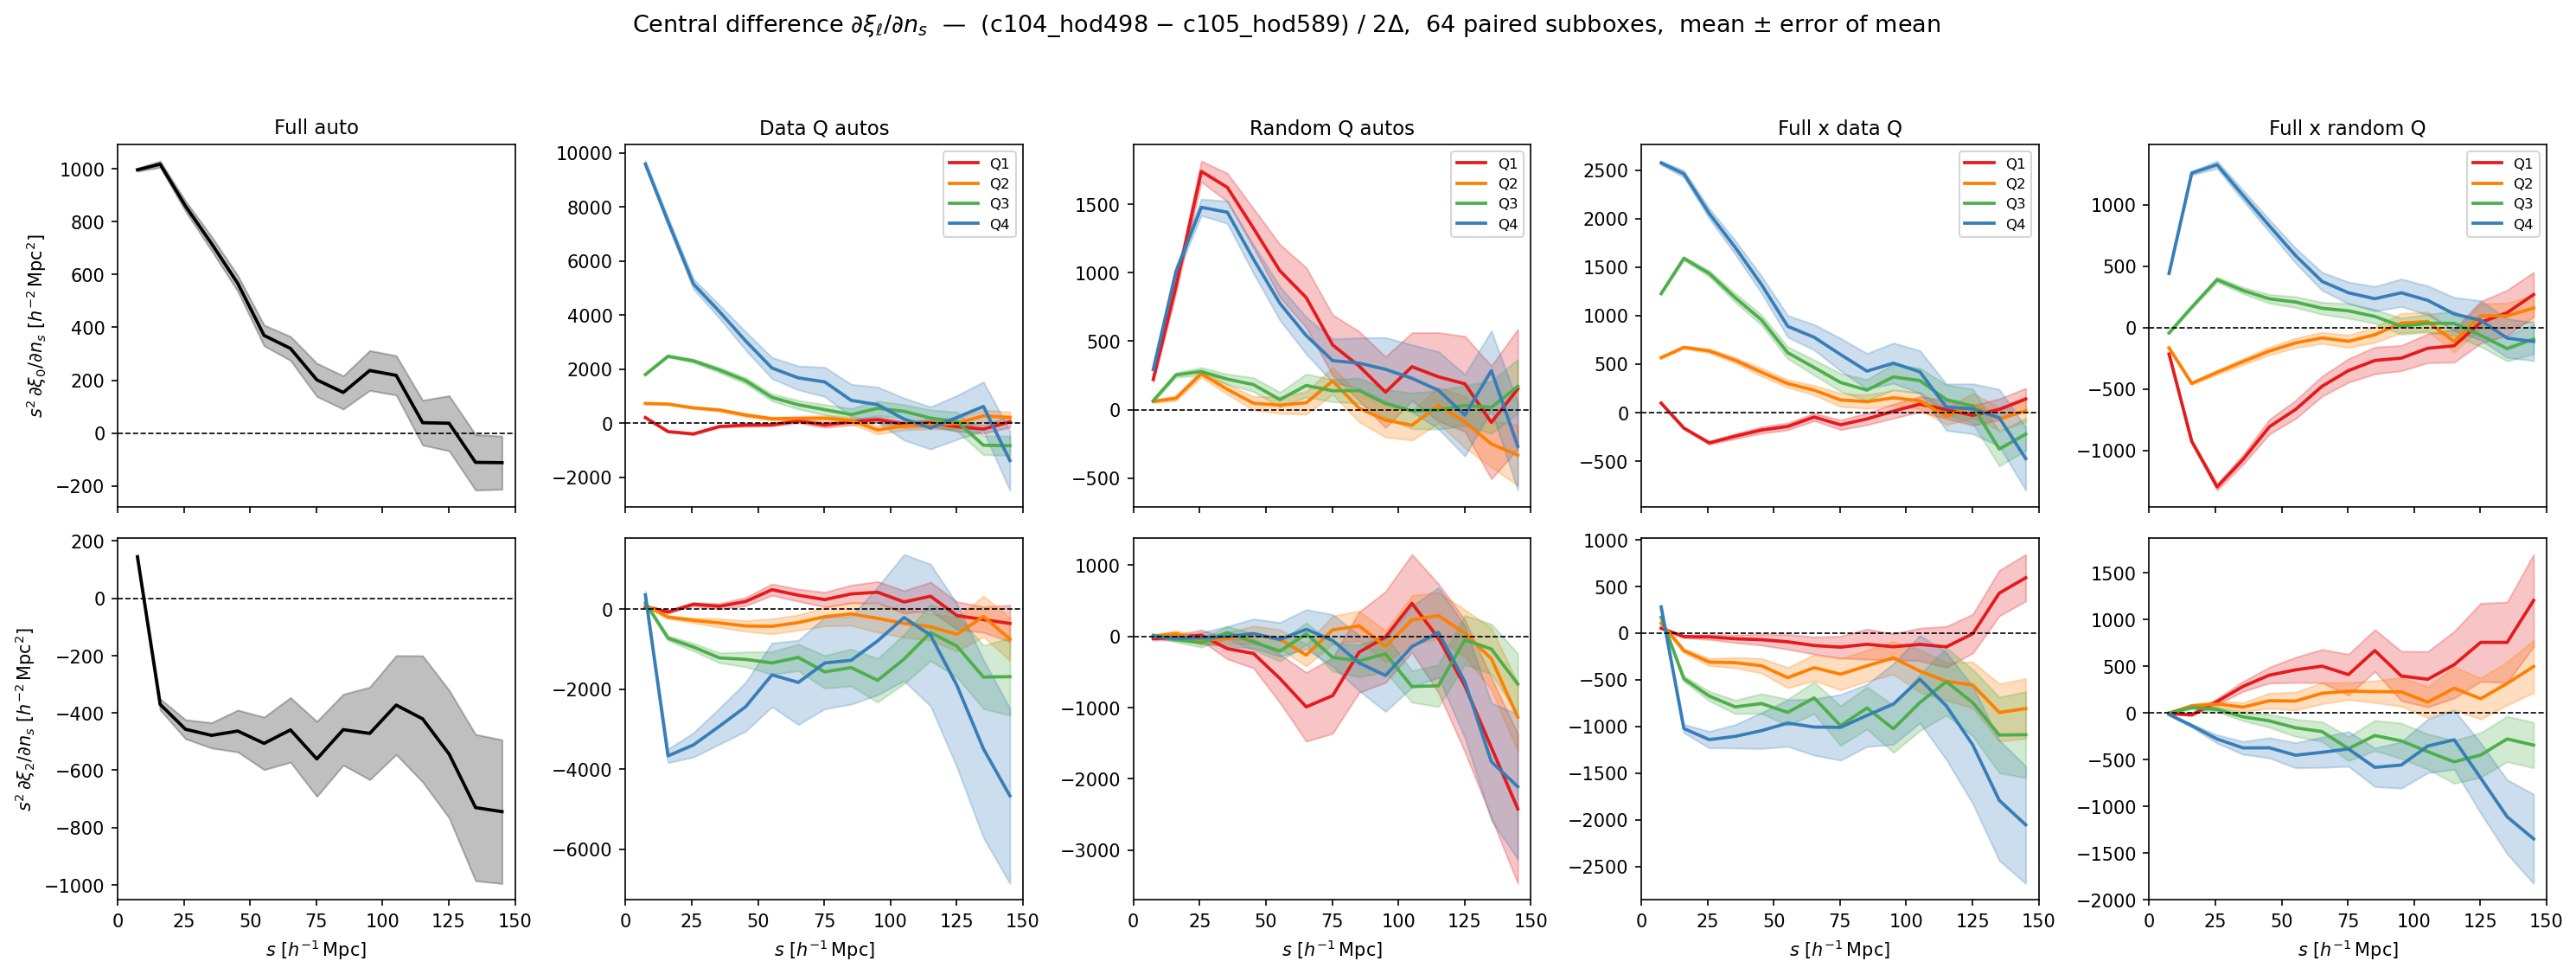
\includegraphics[width=0.49\textwidth]{derivative_ns.png}\hfill
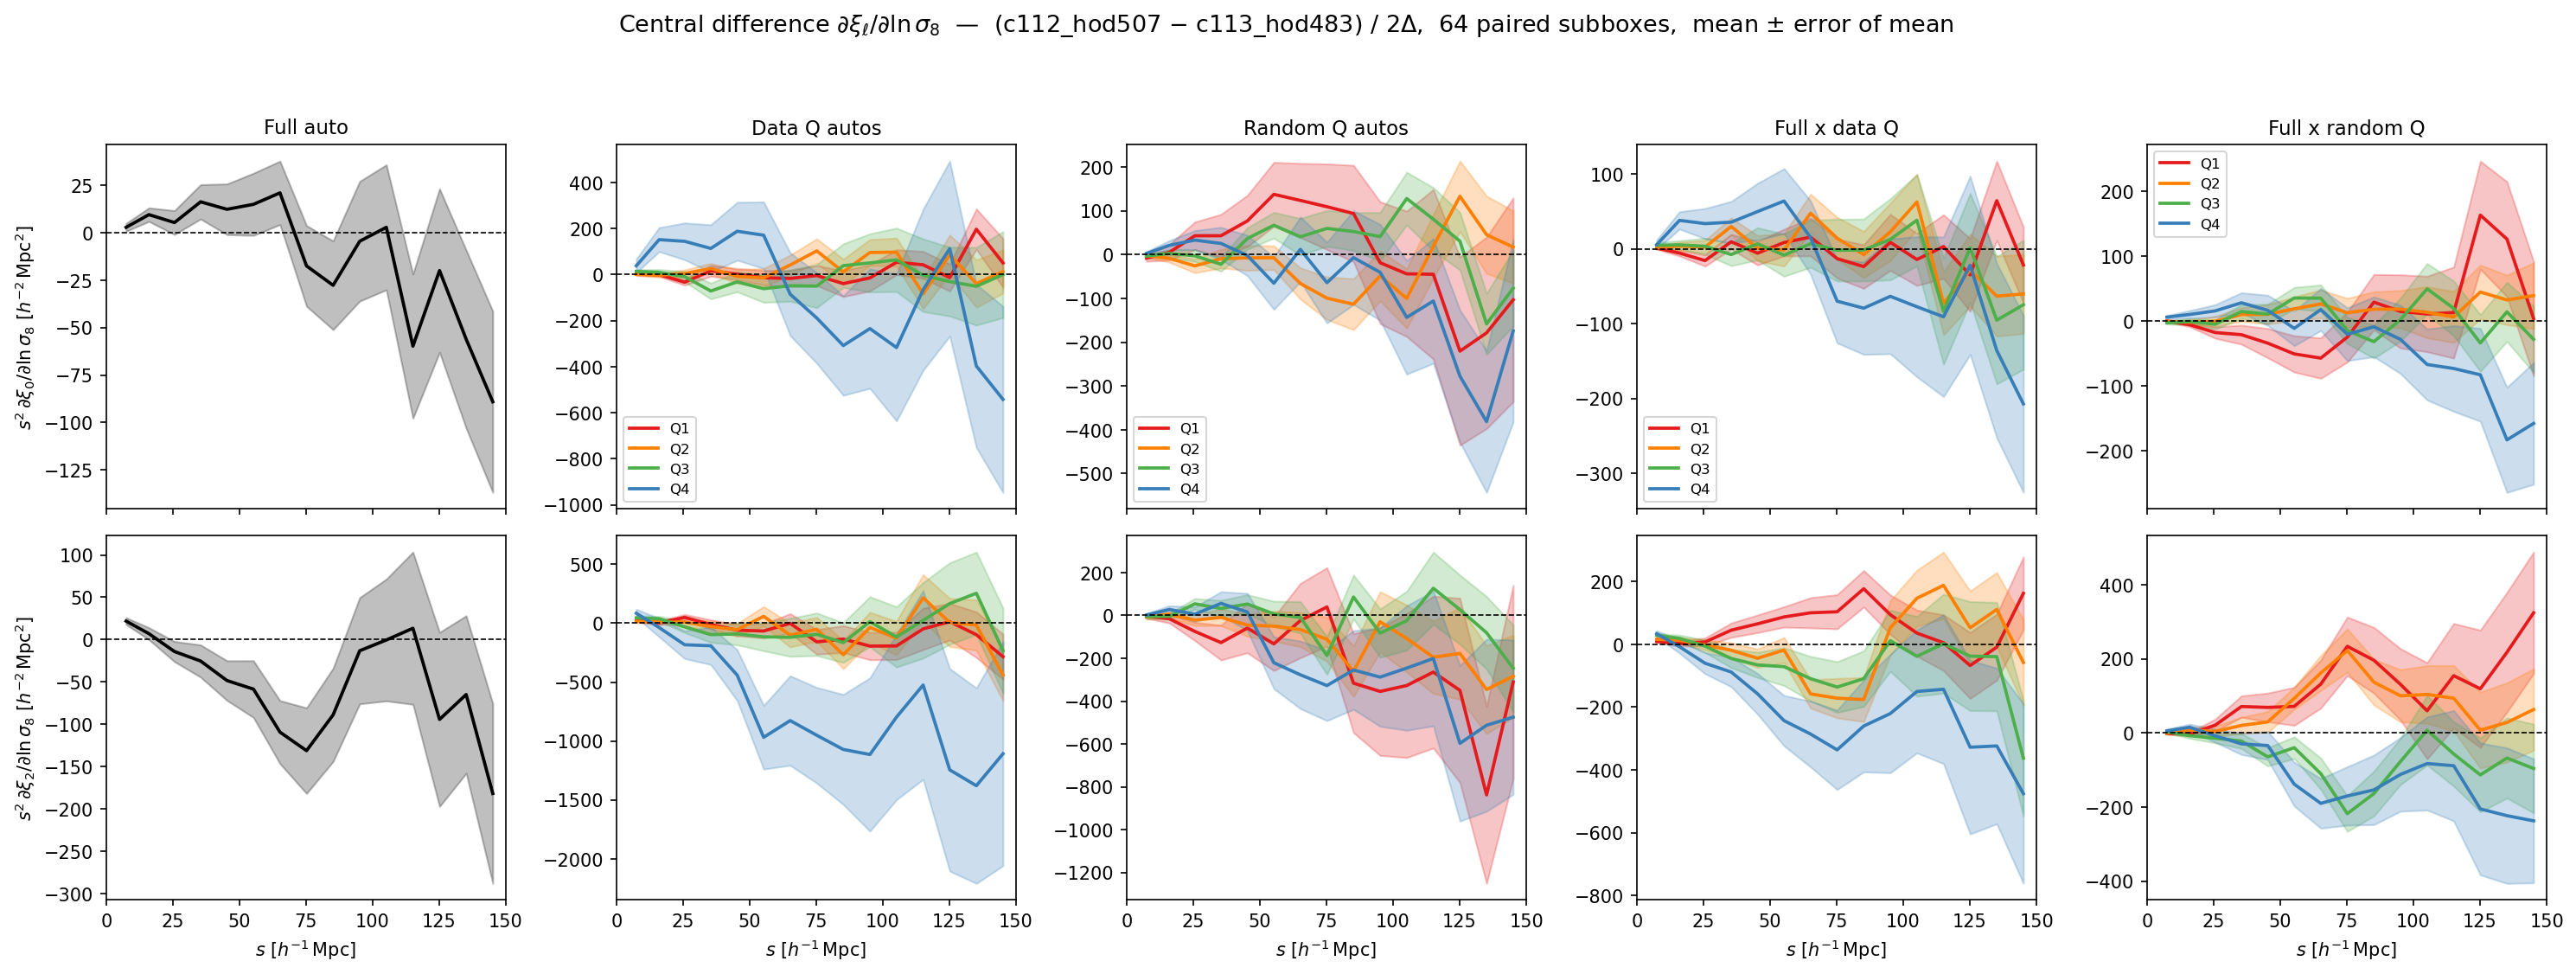
\includegraphics[width=0.49\textwidth]{derivative_lns8.png}
\caption{Paired-subbox central-difference derivatives
$\partial\xi_\ell/\partial\theta$ for $\theta=\ln\omega_b$ (top left),
$\ln\omega_{cdm}$ (top right), $n_s$ (bottom left), $\ln\sigma_8$ (bottom
right).  Columns within each panel: full auto, data quantile autos, random
quantile autos, full$\times$data quantiles, full$\times$random quantiles;
rows: monopole and quadrupole.  Lines are the mean over 64 paired subboxes,
bands the error of the mean.}
\label{fig:derivatives}
\end{figure}

\subsection{Tier~0: phase-matched full-box differences}

A subbox has open boundaries and high shot noise.  Differencing the
\emph{whole} $2000\Mpch$ box instead,
\begin{equation}
\frac{\partial \xivec}{\partial\theta}
=
\frac{\xivec(\theta+\Delta\theta)-\xivec(\theta-\Delta\theta)}
{2\,\Delta\theta},
\qquad
\mathrm{Var}\!\left(\frac{\partial\xi}{\partial\theta}\right)_{\!b}
=
\frac{\mathrm{std}_+^2/n_+ + \mathrm{std}_-^2/n_-}{(2\,\Delta\theta)^2},
\label{eq:fullbox}
\end{equation}
where the noise model uses the scatter over the $n=3$ ASTRA-random
iterations of each fixed box (the only part that does not cancel in the
phase-matched difference).  Figure~\ref{fig:fullboxcompare} compares the
subbox and full-box derivatives through the resulting single-parameter
$\sigma$, evaluated against a common covariance.  For the three
already-clean parameters the two methods agree to $\approx 3\%$
(consistency check); for $\sigma_8$ the full-box derivative removes the
derivative \emph{noise} that had dominated the subbox estimate, tightening
$\sigma(\ln\sigma_8)$ by $\sim 1.8\times$ and reducing its noise share from
$79\%$ to $\approx 0\%$.  Tier~0 fixes derivative noise but \emph{not} the
HOD contamination bias of Section~\ref{sec:sims}.

\begin{figure}[ht]
\centering
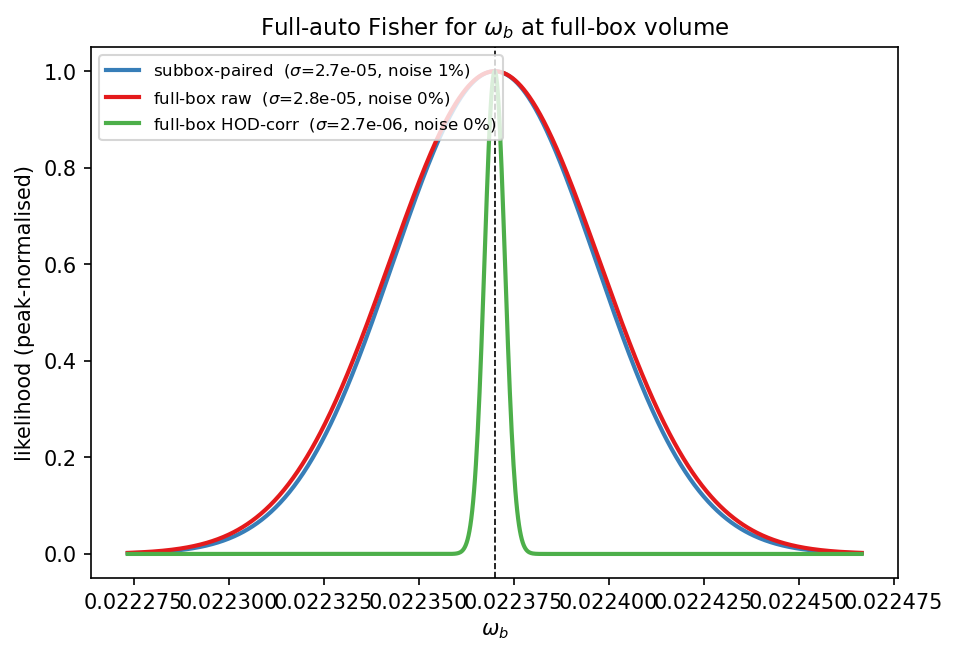
\includegraphics[width=0.49\textwidth]{fisher_fullbox_compare_lnwb.png}\hfill
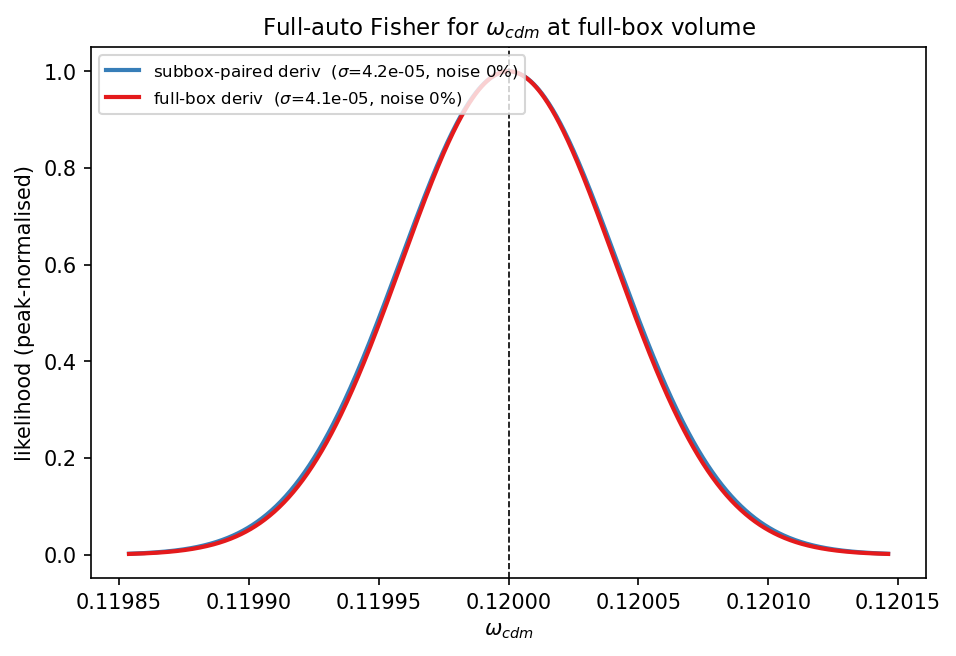
\includegraphics[width=0.49\textwidth]{fisher_fullbox_compare_lnwc.png}\\[4pt]
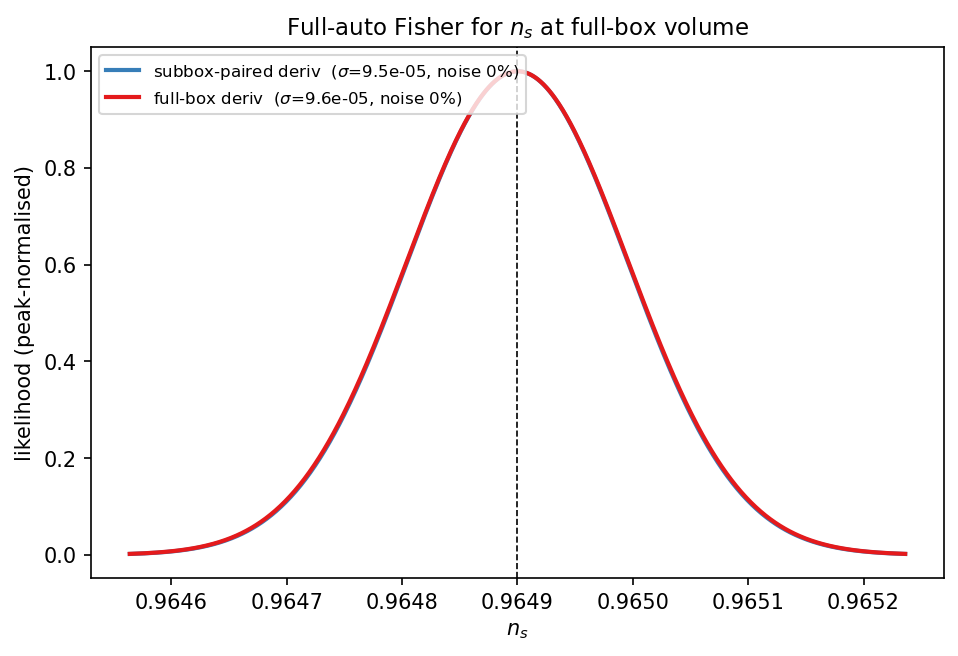
\includegraphics[width=0.49\textwidth]{fisher_fullbox_compare_ns.png}\hfill
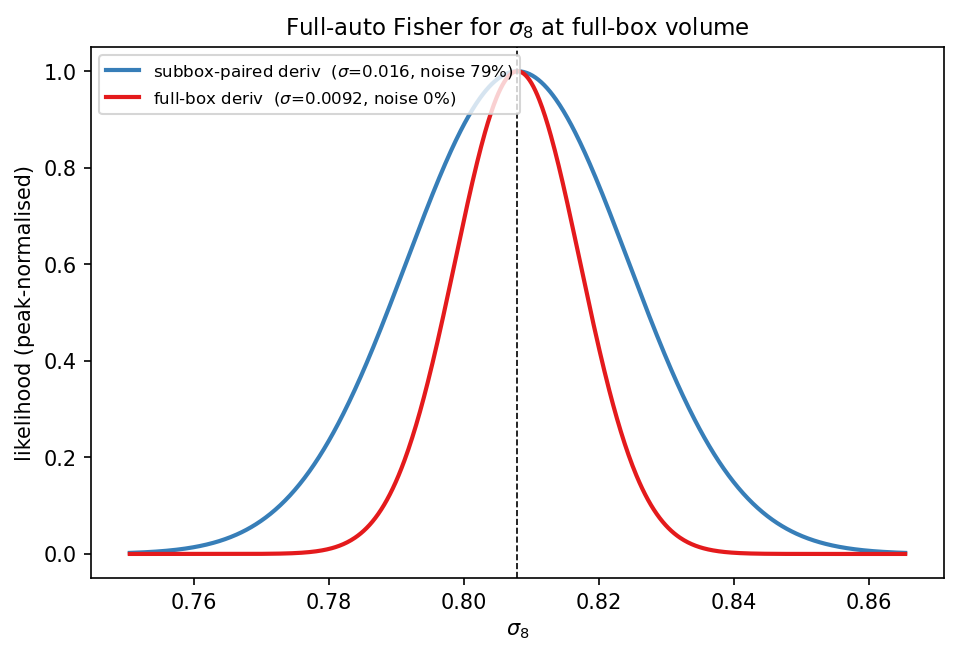
\includegraphics[width=0.49\textwidth]{fisher_fullbox_compare_lns8.png}\\[4pt]
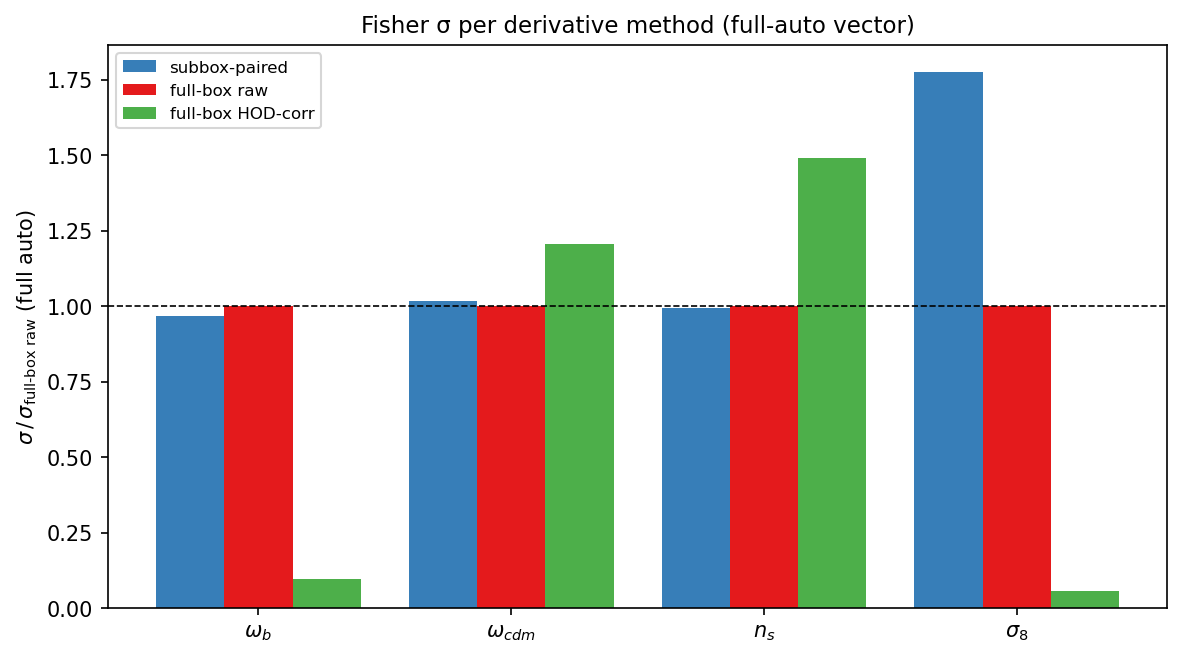
\includegraphics[width=0.7\textwidth]{fisher_fullbox_compare_summary.png}
\caption{Tier~0: subbox vs.\ full-box derivative for each parameter (and
summary, bottom).  The two derivative sources are evaluated against the
same covariance, so only the numerator and noise differ.  The $\sigma_8$
panel shows the noise-driven gain.}
\label{fig:fullboxcompare}
\end{figure}

\subsection{Tier~1: explicit HOD-contamination subtraction}

To remove the contamination \emph{bias}, the HOD response
$\partial\xi/\partial\theta_{\rm HOD}$ is measured by regressing the
full-box $\xi$ on the 12 standardised HOD parameters across $\sim 50$ extra
fiducial-cosmology HOD draws, and the contamination of each pair is
subtracted,
\begin{equation}
\left.\frac{\partial\xivec}{\partial\theta}\right|_{\rm corr}
=
\left.\frac{\partial\xivec}{\partial\theta}\right|_{\rm raw}
-
\frac{\Delta\boldsymbol{\theta}_{\rm HOD}\cdot
\mathsf{G}}{2\,\Delta\theta},
\qquad
\mathsf{G}=\frac{\partial\xivec}{\partial\boldsymbol{\theta}_{\rm HOD}},
\label{eq:hodcorr}
\end{equation}
where $\Delta\boldsymbol{\theta}_{\rm HOD}$ is the measured HOD-parameter
mismatch between the two catalogs of the pair.
Figure~\ref{fig:hodcontam} shows the raw, contamination, and corrected
full-auto derivatives.  The contamination is a large, smooth, sign-changing
tilt comparable to or larger than the raw derivative, confirming the
derivatives were heavily contaminated.  As a physical check, linear theory
gives $\partial\xi/\partial\ln\sigma_8 = 2\xi$ for the full sample; the
raw full-box $\sigma_8$ derivative is only $11\%$ of $2\xi$ (the HOD
mismatch had cancelled most of the signal), while the corrected derivative
recovers $136\%$ of $2\xi$ --- back in the right regime.

\begin{figure}[ht]
\centering
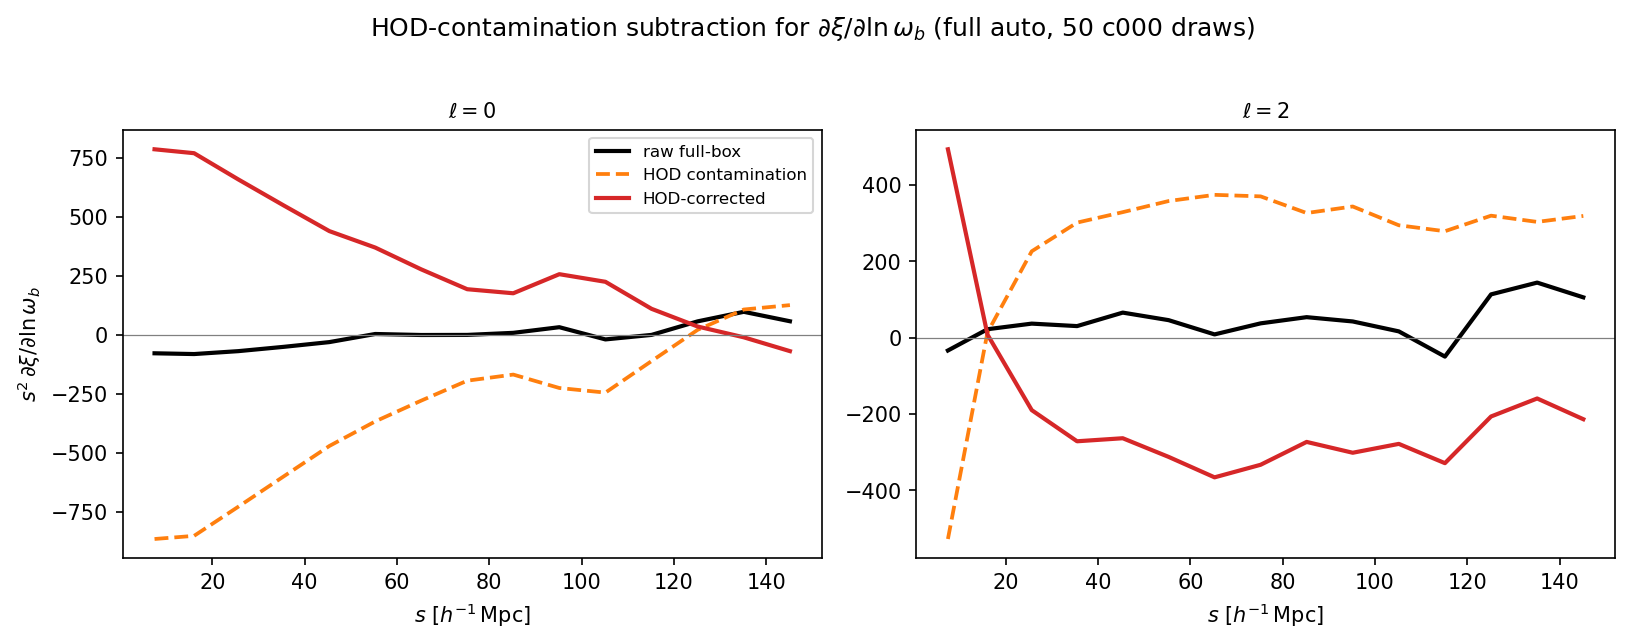
\includegraphics[width=0.49\textwidth]{hod_contamination_lnwb.png}\hfill
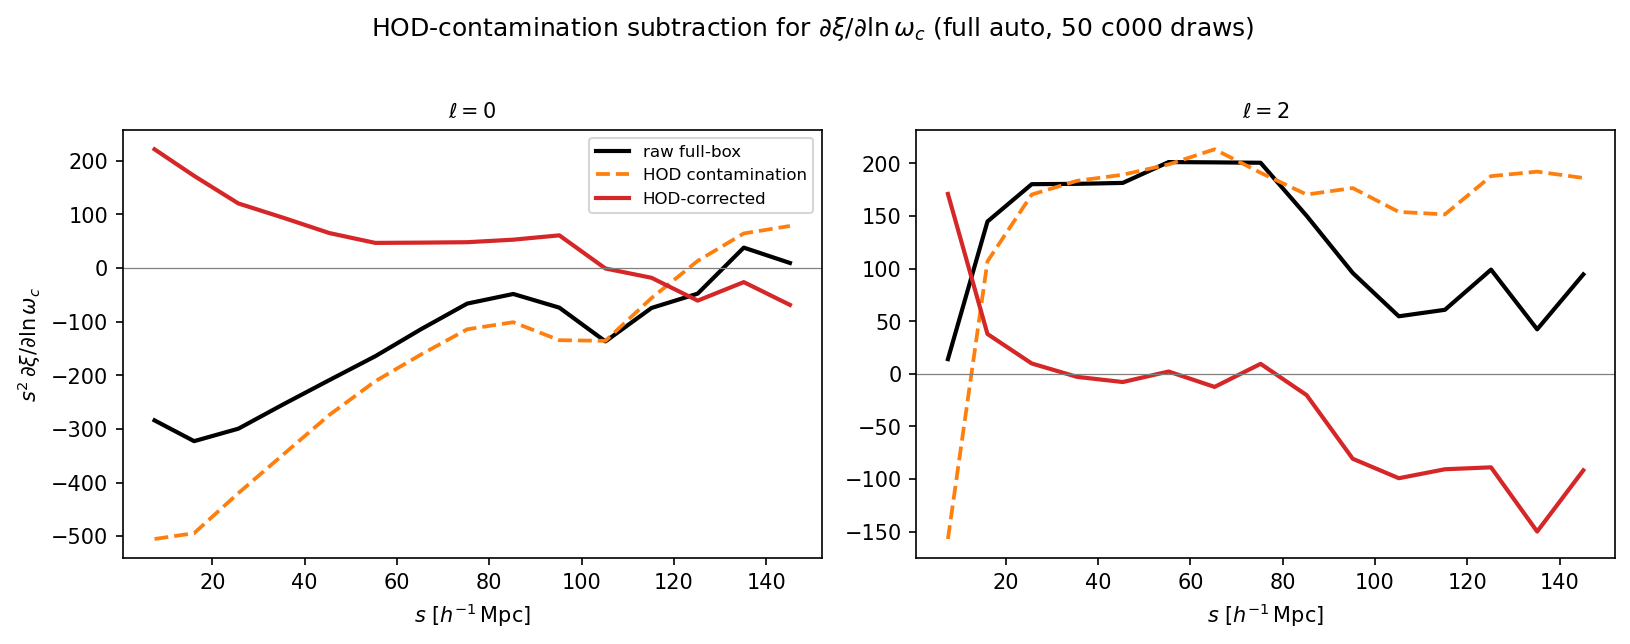
\includegraphics[width=0.49\textwidth]{hod_contamination_lnwc.png}\\[4pt]
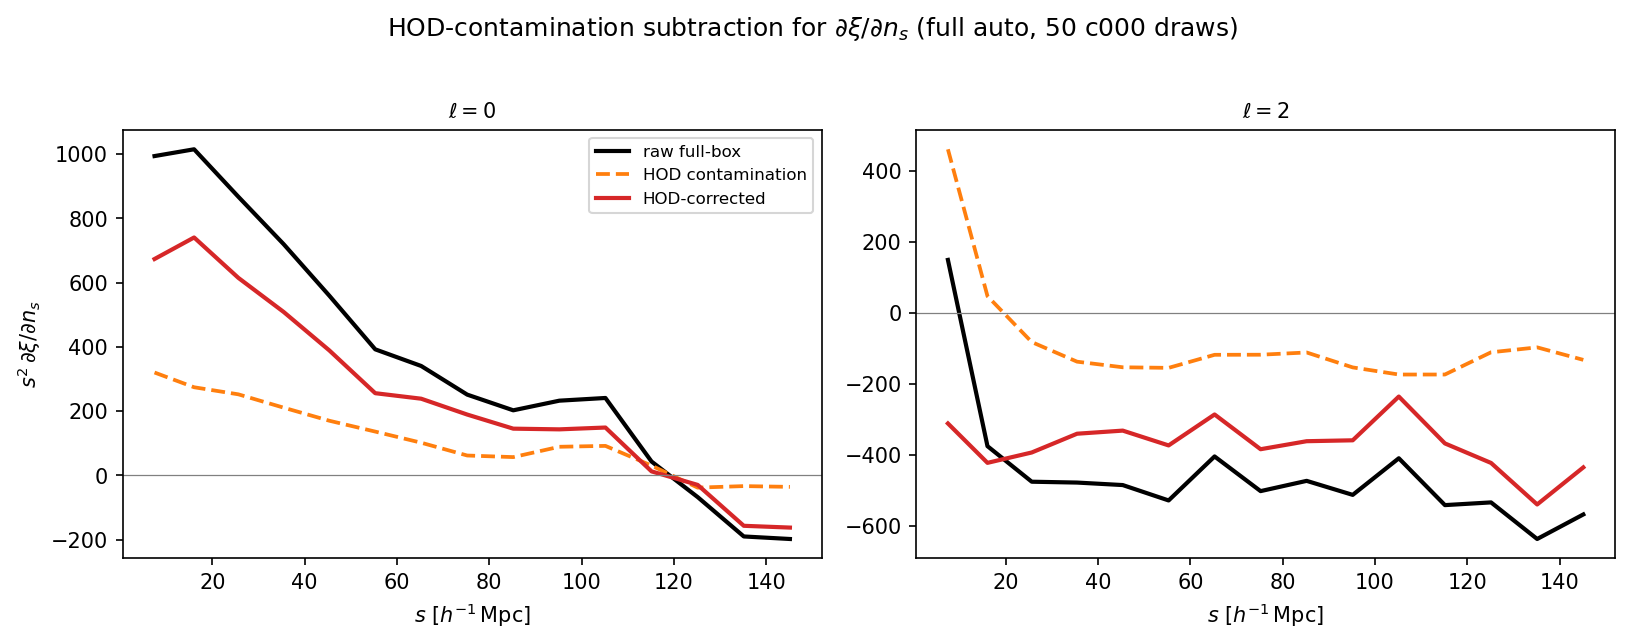
\includegraphics[width=0.49\textwidth]{hod_contamination_ns.png}\hfill
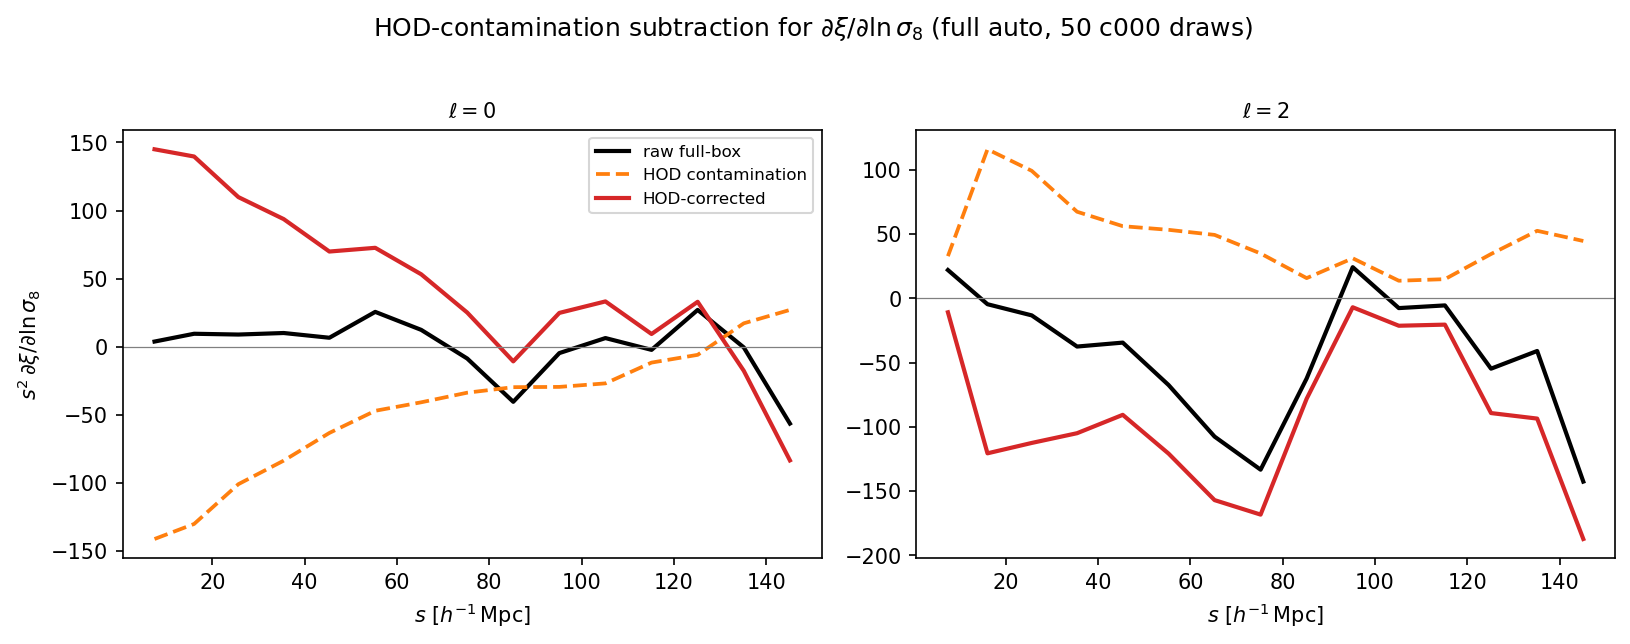
\includegraphics[width=0.49\textwidth]{hod_contamination_lns8.png}
\caption{Tier~1 HOD-contamination subtraction, Eq.~(\ref{eq:hodcorr}),
for the full-sample auto-correlation ($\ell=0$ and $\ell=2$).  Black: raw
full-box derivative; orange dashed: modelled HOD contamination; red:
corrected derivative.}
\label{fig:hodcontam}
\end{figure}

\section{Covariance}
\label{sec:covariance}

The covariance enters Eq.~(\ref{eq:fisher}) as the normalised correlation
matrix $R_{ij}=\mathsf{C}_{ij}/\sqrt{\mathsf{C}_{ii}\mathsf{C}_{jj}}$ shown
in Fig.~\ref{fig:covariances}.  Neighbouring separation bins are strongly
correlated, with the correlation length growing toward large $s$.  The full
auto and the full$\times$data~Q4 blocks are nearly perfectly correlated
(the redundancy discussed below), whereas the full$\times$random~Q1 block
is \emph{anti}-correlated with them --- the only genuinely complementary
information among those three.

\begin{figure}[ht]
\centering
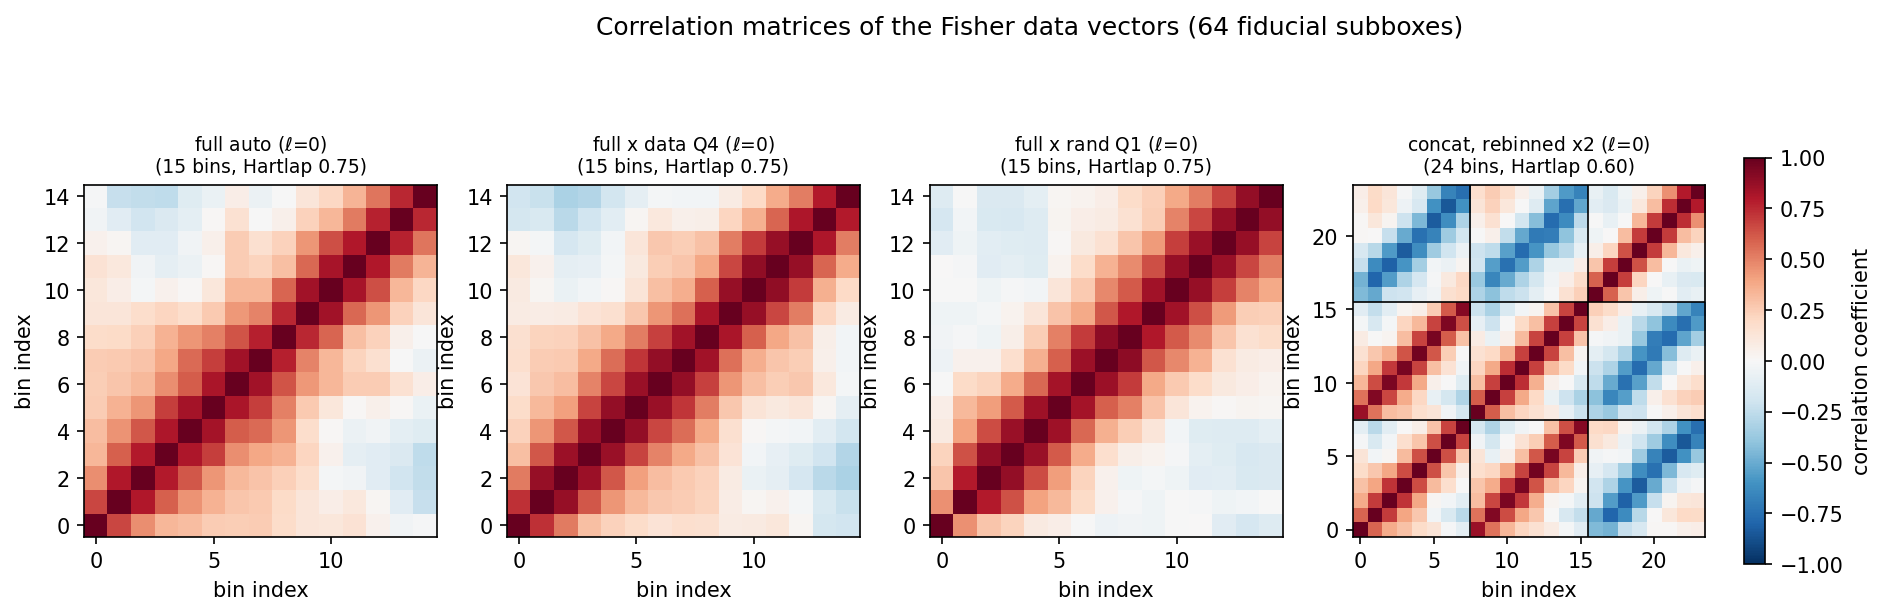
\includegraphics[width=\textwidth]{fisher_covariances.png}
\caption{Correlation matrices of representative data vectors, estimated
from the fiducial subboxes.  Panel titles give the number of bins and the
Hartlap factor $(N-p-2)/(N-1)$.}
\label{fig:covariances}
\end{figure}

\paragraph{Pooling across cosmologies.}
Estimating $\mathsf{C}$ from the 64 fiducial subboxes alone caps the data
vector at $p<64$ bins; adding the quadrupole to the quantile vectors
exceeds this and drives the Hartlap factor negative.  Since the covariance
varies far more slowly with cosmology than the mean does, we instead pool
the mean-subtracted subboxes across all nine cosmologies,
\begin{equation}
\mathsf{C}_{\rm sub}
=
\frac{1}{N-n_c}\sum_{c=1}^{n_c}\sum_{i=1}^{64}
\big(\xivec_{ci}-\bar{\xivec}_c\big)
\big(\xivec_{ci}-\bar{\xivec}_c\big)^{\!\top},
\qquad N = n_c\times 64 = 576,
\label{eq:pool}
\end{equation}
removing each cosmology's own mean $\bar{\xivec}_c$ so that only
cosmic-variance fluctuations survive.  The full-box covariance is
$\mathsf{C}=\mathsf{C}_{\rm sub}/64$.  With $N=576$ the Hartlap factor stays
$\gtrsim 0.75$ even at $p=144$ bins, so mono$+$quad data and random
quantile vectors fit comfortably.  The caveat is that subboxes tile a
single box per cosmology and share large-scale modes, so the effective
number of independent samples is below 576 --- but this approximation was
already implicit in the 64-subbox estimate.

\section{Joint cosmology\,+\,HOD Fisher}
\label{sec:joint}

Fixing the HOD exactly is optimistic, because the $\sigma_8$ response is
amplitude-like and so degenerate with HOD bias.  We therefore build one
Fisher over the 4 cosmology parameters \emph{and} the 12 HOD parameters and
marginalise the latter,
\begin{equation}
F = \mathsf{D}\,\mathsf{C}^{-1}\mathsf{D}^{\!\top} + F_{\rm prior},
\quad
\mathsf{D}=
\begin{bmatrix}
\partial\xivec/\partial\boldsymbol{\theta}_{\rm cosmo}\ (4\ \text{rows})\\[2pt]
\partial\xivec/\partial\boldsymbol{\theta}_{\rm HOD}\ (12\ \text{rows})
\end{bmatrix},
\quad
F_{\rm prior}=\mathrm{diag}\!\big(\mathbf{0}_4,\ \sigma_{\rm prior}^{-2}\big),
\label{eq:joint}
\end{equation}
where the cosmology rows are the HOD-corrected derivatives
(Eq.~\ref{eq:hodcorr}) and the HOD rows are the regression gradient
$\mathsf{G}$.  The poorly-constrained HOD directions are regularised by a
Gaussian yuan23 prior ($\sigma_{\rm prior}$ = spread of the fiducial HOD
draws), \emph{not} by truncation, which would be an implicit infinite prior
and reintroduce the fixed-HOD optimism.  The conditional cosmology error
inverts the $4\times4$ cosmology block of $\mathsf{D}\mathsf{C}^{-1}
\mathsf{D}^\top$; the marginalised error inverts the full $16\times16$
$F$ and reads off the cosmology block.

Table~\ref{tab:joint} gives the full-auto result.  $n_s$ and $\omega_b$
degrade most under marginalisation because their tight conditional errors
overlap the broadband HOD tilt directions; in fractional terms all four
parameters land at $0.6$--$1.2\%$ from a single $2\Mpch[\mathrm{Gpc}]$ box.
Figure~\ref{fig:jointmarg} shows the degradation, Fig.~\ref{fig:jointconv}
the robustness check (the cosmology errors plateau by $\sim4$ marginalised
HOD directions, so the prior-controlled tail is irrelevant), and
Fig.~\ref{fig:jointellipses} the conditional vs.\ marginalised ellipses.

\begin{table}[ht]
\centering
\begin{tabular}{lcccc}
\toprule
Parameter & $\sigma_{\rm cond}$ (HOD fixed) & $\sigma_{\rm marg}$ (HOD marg.) & degrade & $\sigma_{\rm marg}/\theta_{\rm fid}$ \\
\midrule
$\omega_b$      & $3.08\times10^{-5}$ & $2.49\times10^{-4}$ & $8.1\times$  & $1.1\%$  \\
$\omega_{cdm}$  & $4.88\times10^{-4}$ & $1.01\times10^{-3}$ & $2.1\times$  & $0.85\%$ \\
$n_s$           & $5.78\times10^{-4}$ & $5.89\times10^{-3}$ & $10.2\times$ & $0.61\%$ \\
$\ln\sigma_8$   & $3.18\times10^{-3}$ & $9.31\times10^{-3}$ & $2.9\times$  & $1.15\%$ \\
\bottomrule
\end{tabular}
\caption{Joint Fisher on the full-auto mono$+$quad vector (HOD-corrected
derivatives, 64-subbox covariance scaled to the full box).  Conditional
holds the HOD fixed; marginalised marginalises the 12 HOD nuisances under
the yuan23 prior.}
\label{tab:joint}
\end{table}

\begin{figure}[ht]
\centering
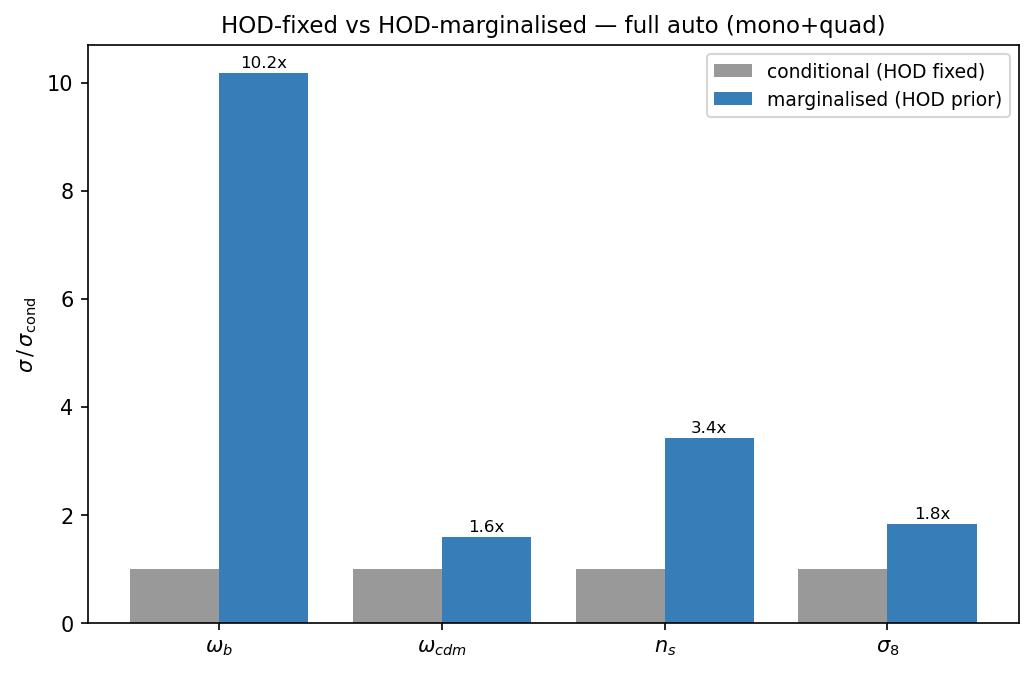
\includegraphics[width=0.49\textwidth]{fisher_joint_marginalisation.png}\hfill
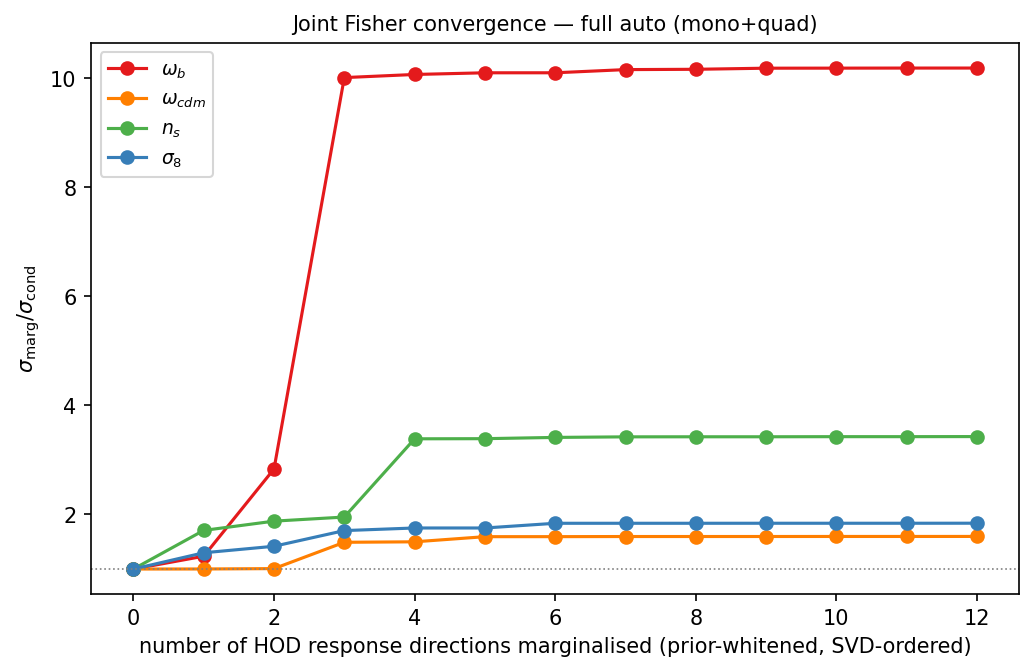
\includegraphics[width=0.49\textwidth]{fisher_joint_convergence.png}
\caption{Left: cosmology errors, HOD-fixed vs.\ HOD-marginalised (the
degradation factors of Table~\ref{tab:joint}).  Right: convergence of the
marginalised error as HOD response directions are marginalised one at a
time (prior-whitened, SVD-ordered); the plateau by $k\approx4$ shows the
HOD response is effectively low-rank.}
\label{fig:jointmarg}
\label{fig:jointconv}
\end{figure}

\begin{figure}[ht]
\centering
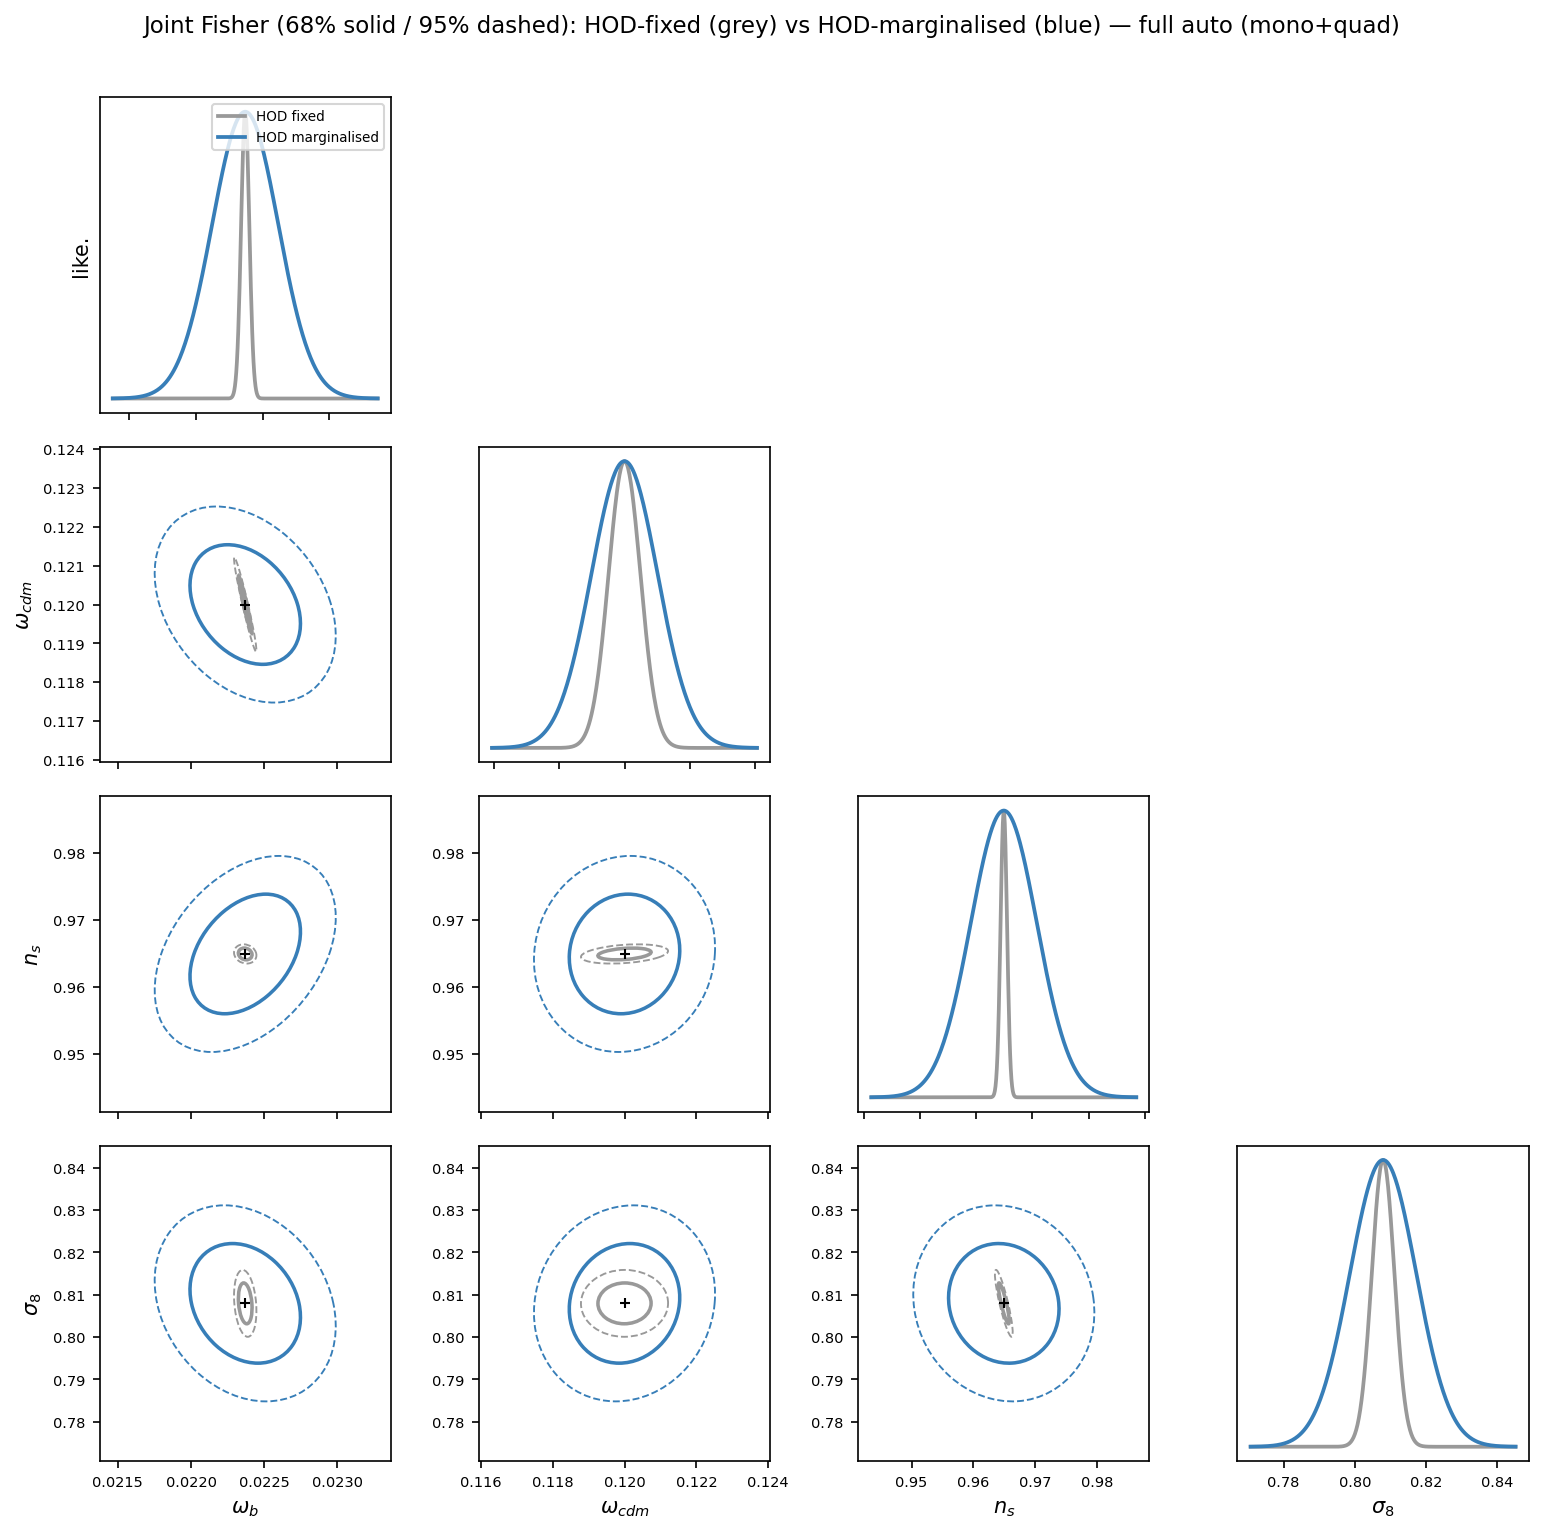
\includegraphics[width=\textwidth]{fisher_joint_ellipses.png}
\caption{Joint Fisher $68\%$/$95\%$ ellipses in physical units: HOD-fixed
(grey) vs.\ HOD-marginalised (blue).  The blue ellipses dwarf the grey and
tilt to show the cosmology--cosmology degeneracies that HOD marginalisation
opens up.}
\label{fig:jointellipses}
\end{figure}

\section{Which data vector? Quadrupole and random quantiles}
\label{sec:vectors}

With the pooled covariance (Eq.~\ref{eq:pool}) lifting the Hartlap limit, we
can ask which statistics carry independent information \emph{after} HOD
marginalisation.  Table~\ref{tab:vectors} compares vectors that share the
same monopole binning and simply add the quadrupole.

\begin{table}[ht]
\centering
\begin{tabular}{lcccccc}
\toprule
Data vector & $p$ & Hartlap & $\sigma(\omega_b)$ & $\sigma(\omega_{cdm})$ & $\sigma(n_s)$ & $\sigma(\sigma_8)$ \\
\midrule
full auto (mono$+$quad)          & 30 & 0.95 & $2.18$ & $9.31$ & $52.3$ & $80.4$ \\
data Q autos (mono)              & 32 & 0.94 & $1.94$ & $7.53$ & $29.9$ & $86.1$ \\
data Q autos (mono$+$quad)       & 64 & 0.89 & $1.46$ & $5.51$ & $18.1$ & $54.5$ \\
full$+$data Q autos (mono)       & 40 & 0.93 & $1.68$ & $5.80$ & $24.0$ & $68.3$ \\
\textbf{full$+$data Q autos (mono$+$quad)} & 80 & 0.86 & $\mathbf{1.14}$ & $\mathbf{4.47}$ & $\mathbf{15.5}$ & $\mathbf{46.0}$ \\
\bottomrule
\end{tabular}
\caption{HOD-marginalised $\sigma$ (units: $\omega_b,\omega_{cdm}$ in
$10^{-4}$; $n_s$ in $10^{-4}$; $\sigma_8$ in $10^{-4}$), pooled 576-sample
covariance, HOD-corrected derivatives.  Adding the quadrupole at fixed
monopole binning tightens every parameter by $1.3$--$1.65\times$; the
earlier finding that ``the quadrupole adds almost nothing'' was a
Hartlap-budget artifact of the 64-subbox covariance.}
\label{tab:vectors}
\end{table}

The full set of marginalised constraints by data vector is shown in the
corner plot of Fig.~\ref{fig:vectorellipses}.  Two robust conclusions:
the quadrupole carries real, largely independent information once it is not
crowded out of the Hartlap budget; and the ASTRA environment split itself
helps --- the quantile autos beat the full auto, and combining the full
sample with the quantiles is tighter still.

\begin{figure}[ht]
\centering
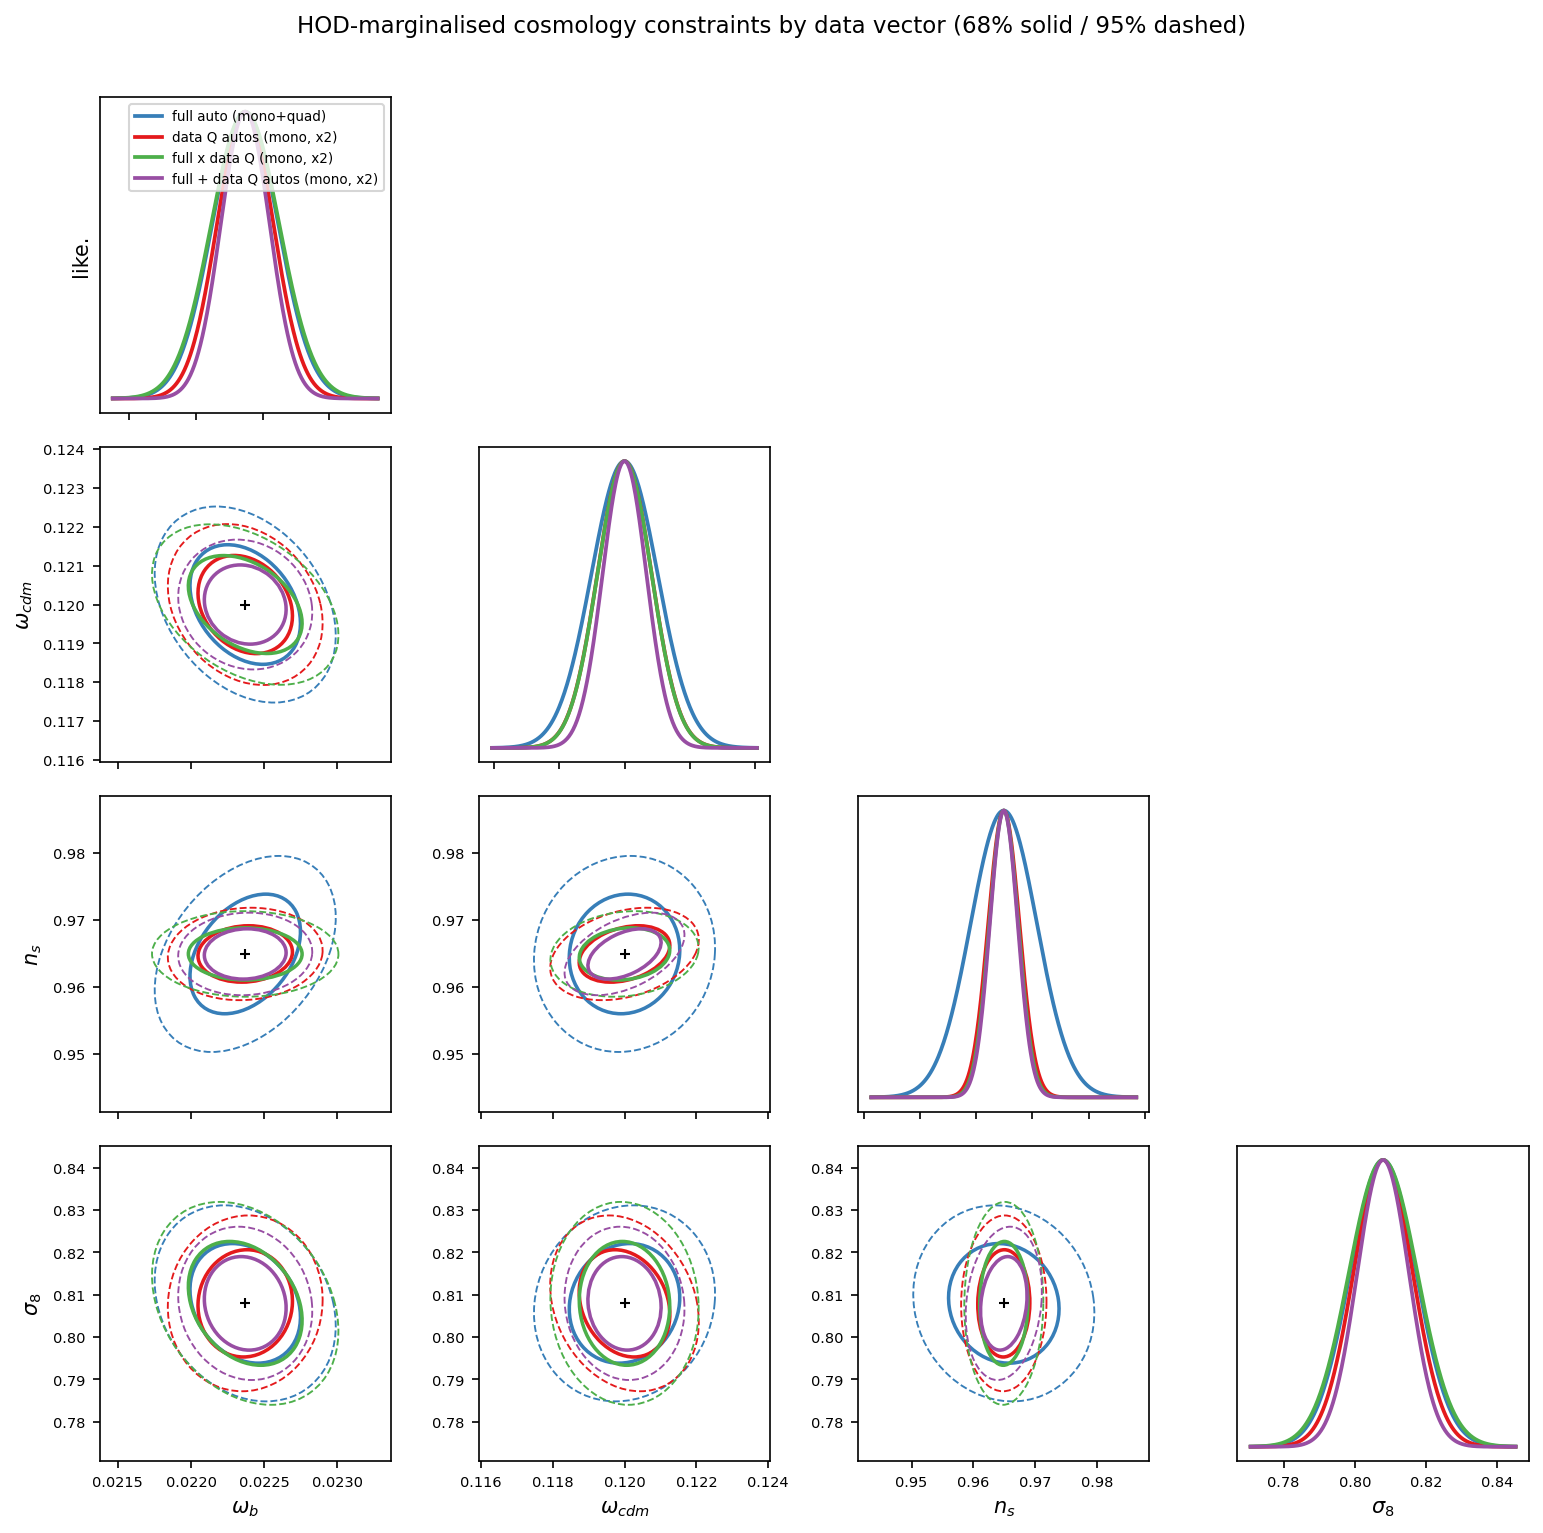
\includegraphics[width=\textwidth]{fisher_joint_ellipses_vectors.png}
\caption{HOD-marginalised $68\%$/$95\%$ cosmology constraints by data
vector.  Vectors that add the ASTRA quantiles and the quadrupole shrink the
ellipses relative to the full-auto baseline.}
\label{fig:vectorellipses}
\end{figure}

The single-parameter view of the same comparison is shown in
Fig.~\ref{fig:gaussians}, where each candidate data vector is drawn as a
one-parameter Fisher Gaussian (Eq.~\ref{eq:gauss}) around the fiducial
value, for one subbox volume and for the full box.  These reproduce the
per-vector ranking parameter by parameter and make the relative widths
directly legible.

\begin{figure}[ht]
\centering
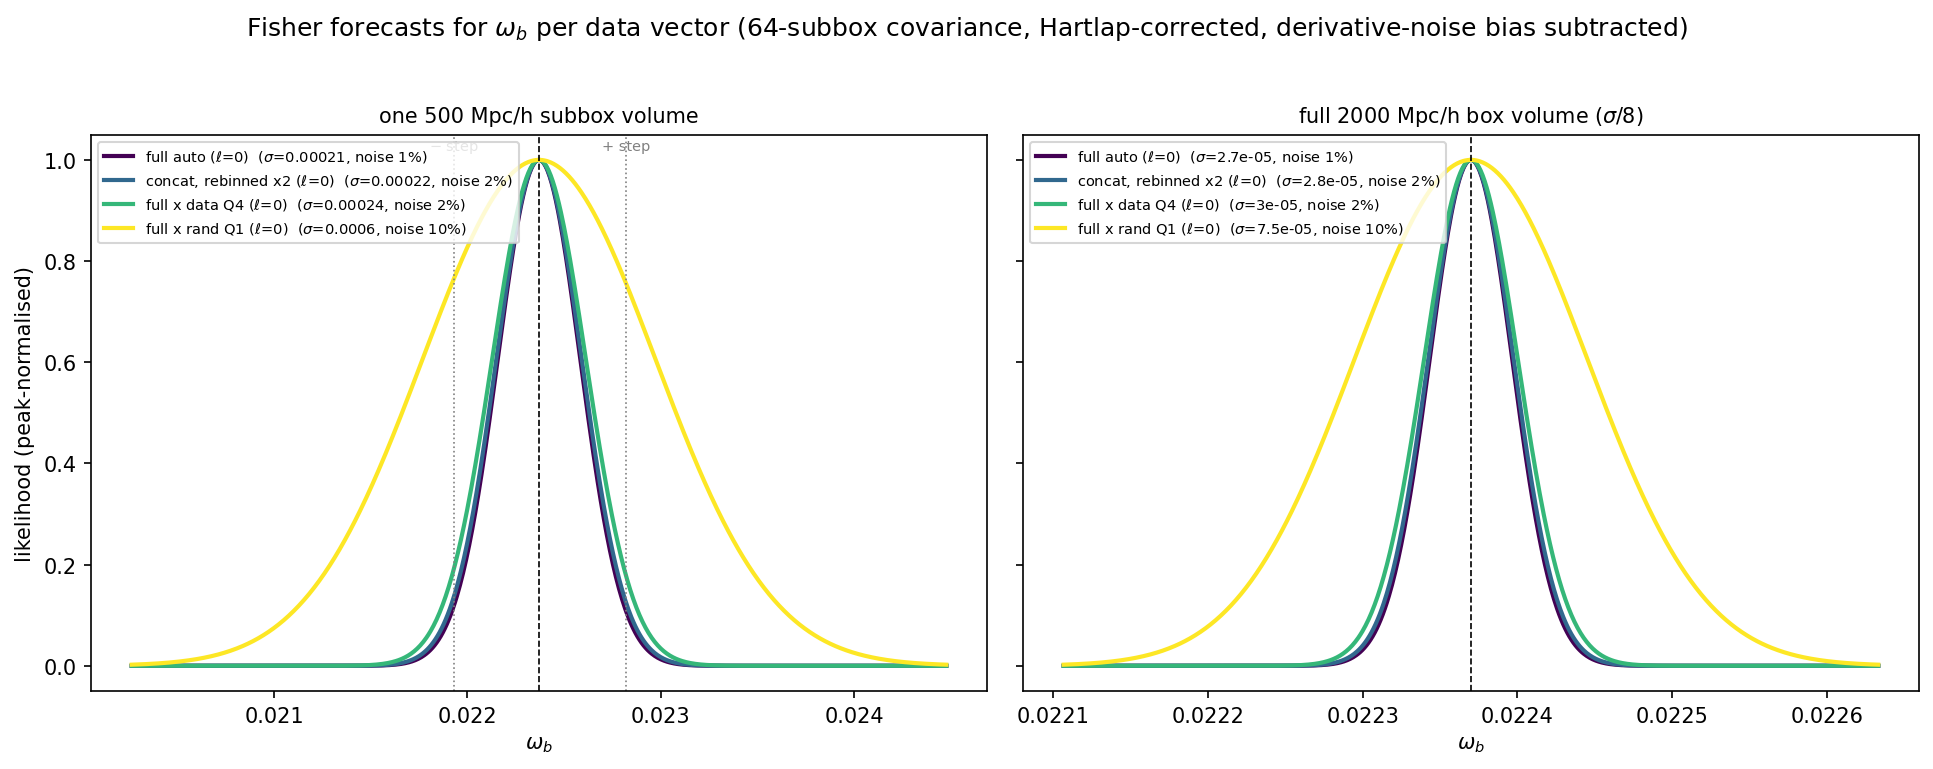
\includegraphics[width=0.49\textwidth]{fisher_gaussians_lnwb.png}\hfill
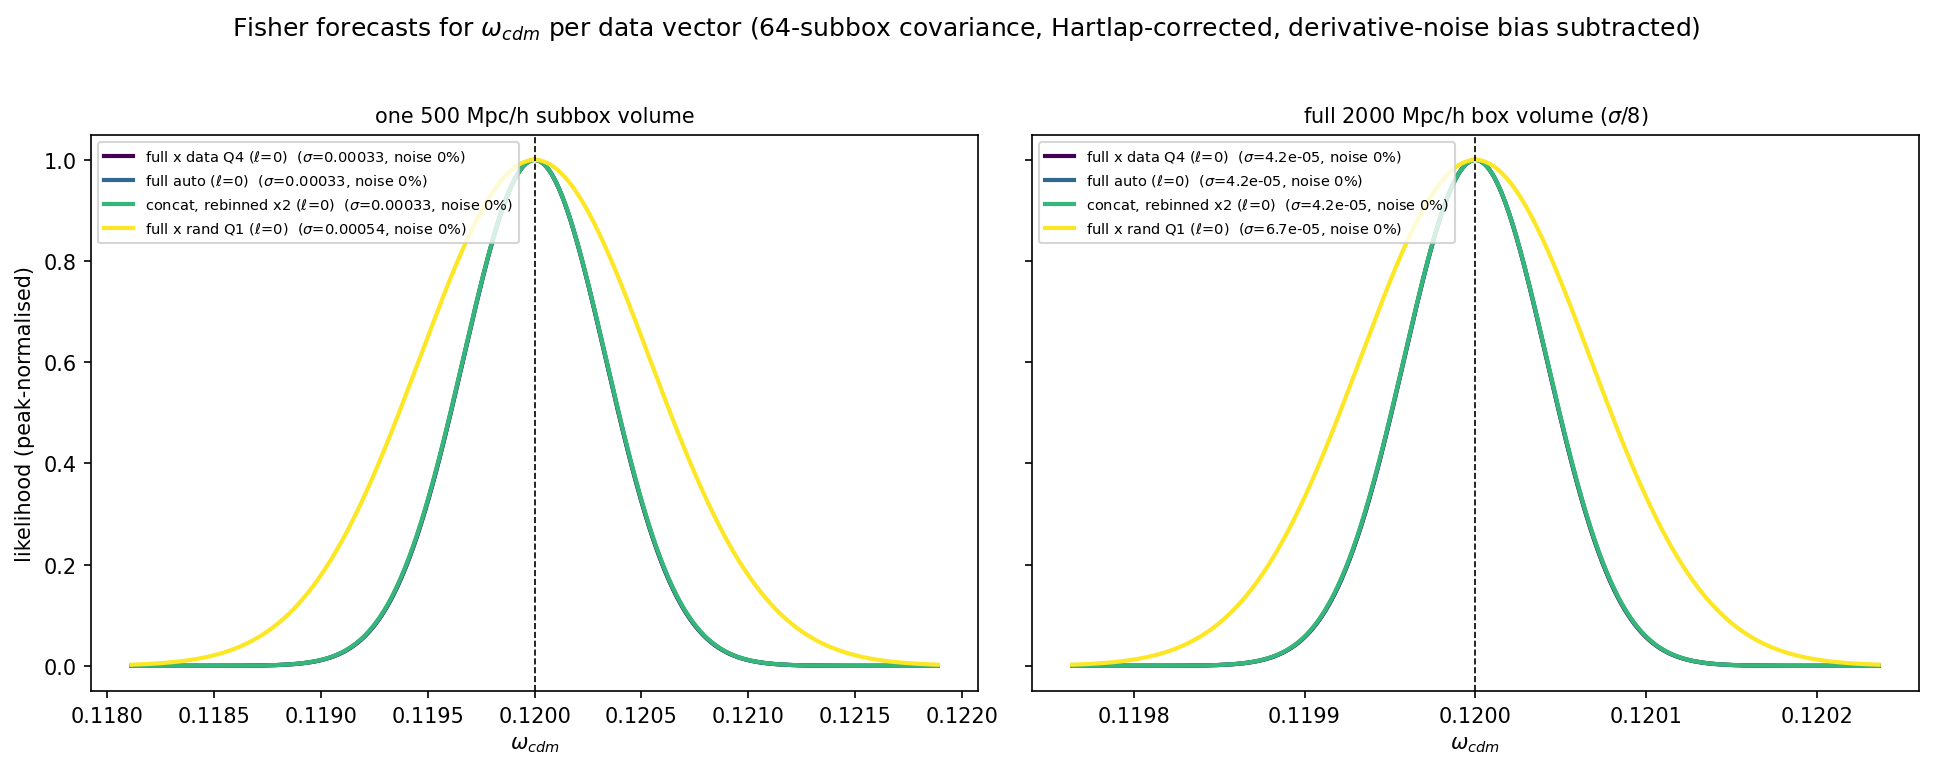
\includegraphics[width=0.49\textwidth]{fisher_gaussians_lnwc.png}\\[4pt]
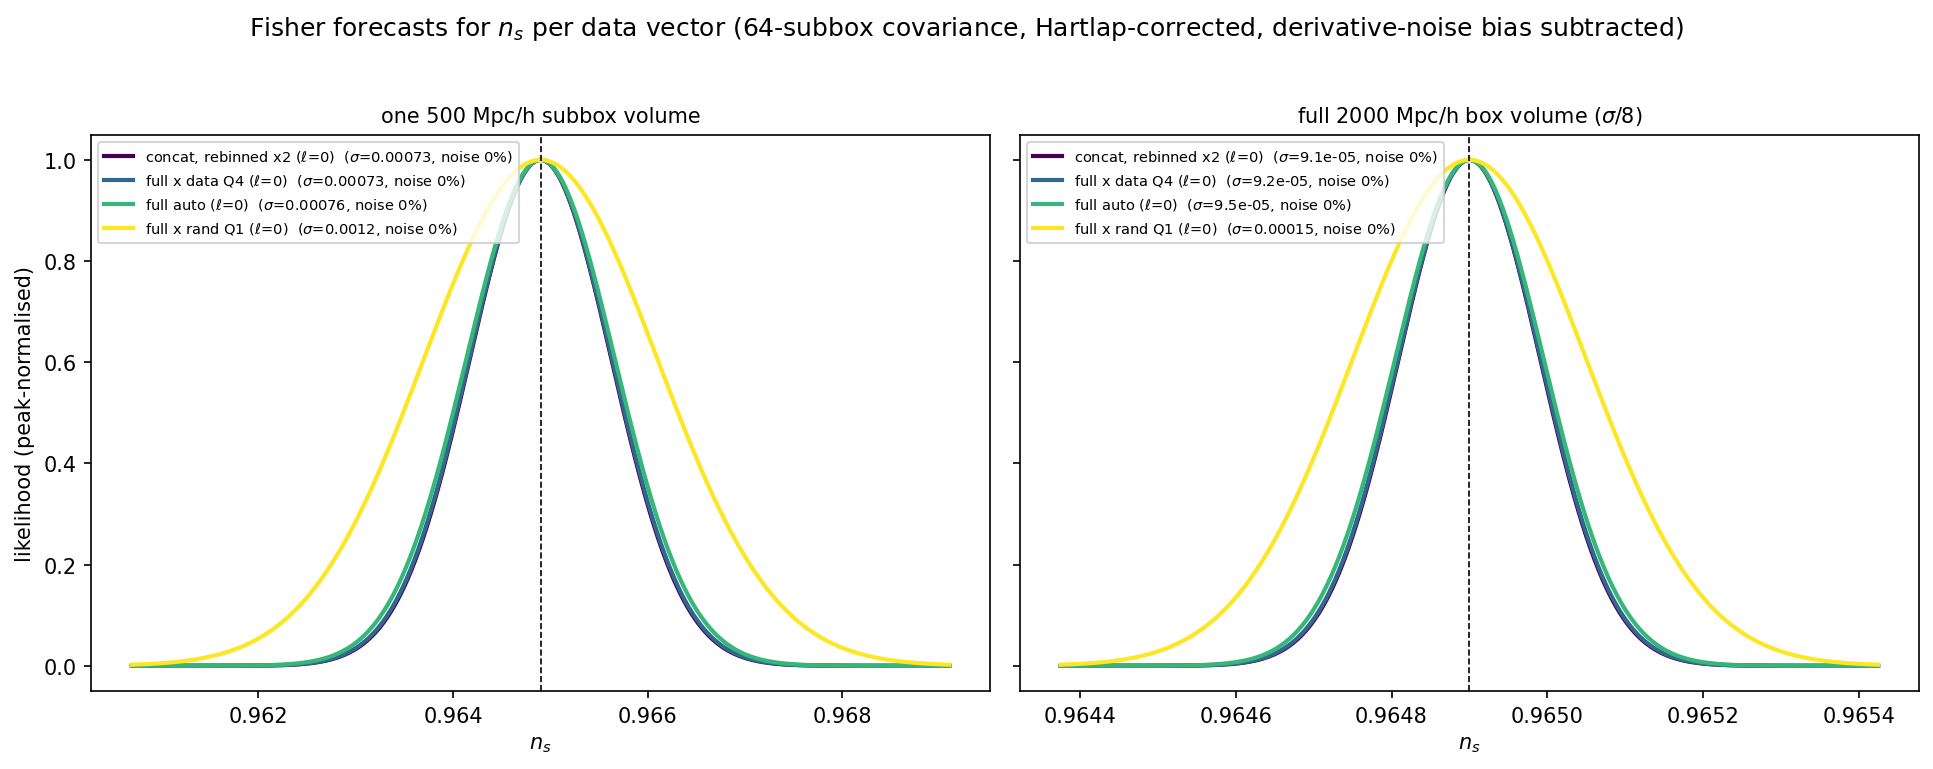
\includegraphics[width=0.49\textwidth]{fisher_gaussians_ns.png}\hfill
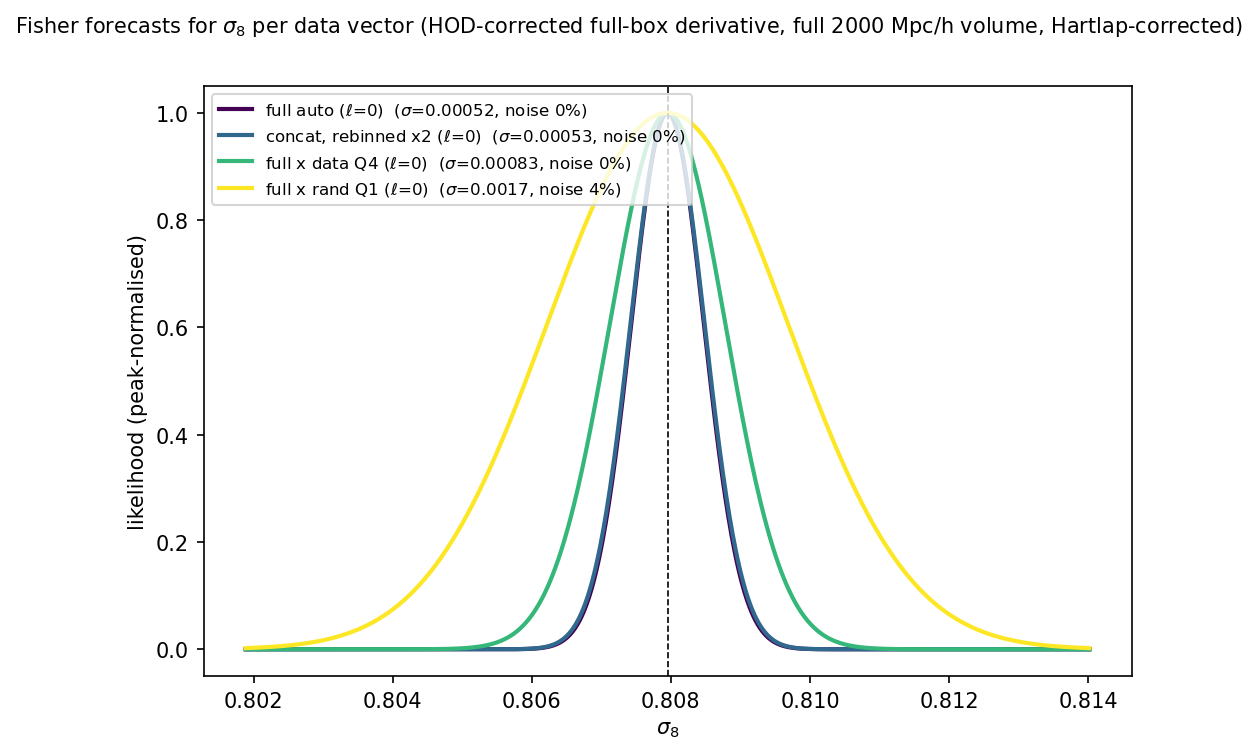
\includegraphics[width=0.49\textwidth]{fisher_gaussians_lns8.png}
\caption{Single-parameter Fisher likelihoods (Eq.~\ref{eq:gauss}),
normalised to unit peak, for a selection of data vectors and each of the
four parameters: $\ln\omega_b$ (top left), $\ln\omega_{cdm}$ (top right),
$n_s$ (bottom left), $\ln\sigma_8$ (bottom right).  Narrower is more
constraining.}
\label{fig:gaussians}
\end{figure}

\section{Global response model}
\label{sec:global}

The contamination subtraction of Section~\ref{sec:derivatives} is a
first-order patch.  The cleaner route, enabled by the $\sim 500$ existing
HOD draws \emph{per} cosmology, is to run $\sim 50$ maximin-selected draws
in every cosmology and fit one global linear response across all runs,
\begin{equation}
\xivec(\boldsymbol{\theta})
\;\approx\;
\xivec_0
+ \sum_p a_p\,\theta_{{\rm cosmo},p}
+ \sum_q b_q\,\theta_{{\rm HOD},q}.
\label{eq:global}
\end{equation}
Because the HOD term absorbs the HOD variation explicitly, the cosmology
coefficients $a_p$ \emph{are} the HOD-marginalised cosmology derivatives:
the cross-cosmology HOD mismatch no longer contaminates them, and (all runs
sharing \texttt{ph000}) cosmic variance cancels in $a_p$.  The HOD
coefficients $b_q$ give the gradient $\mathsf{G}$.  This single fit replaces
the Tier~0$+$Tier~1 chain; the finite-difference derivatives are retained
only as a cross-check (Fig.~\ref{fig:globalfd}).

\begin{figure}[ht]
\centering
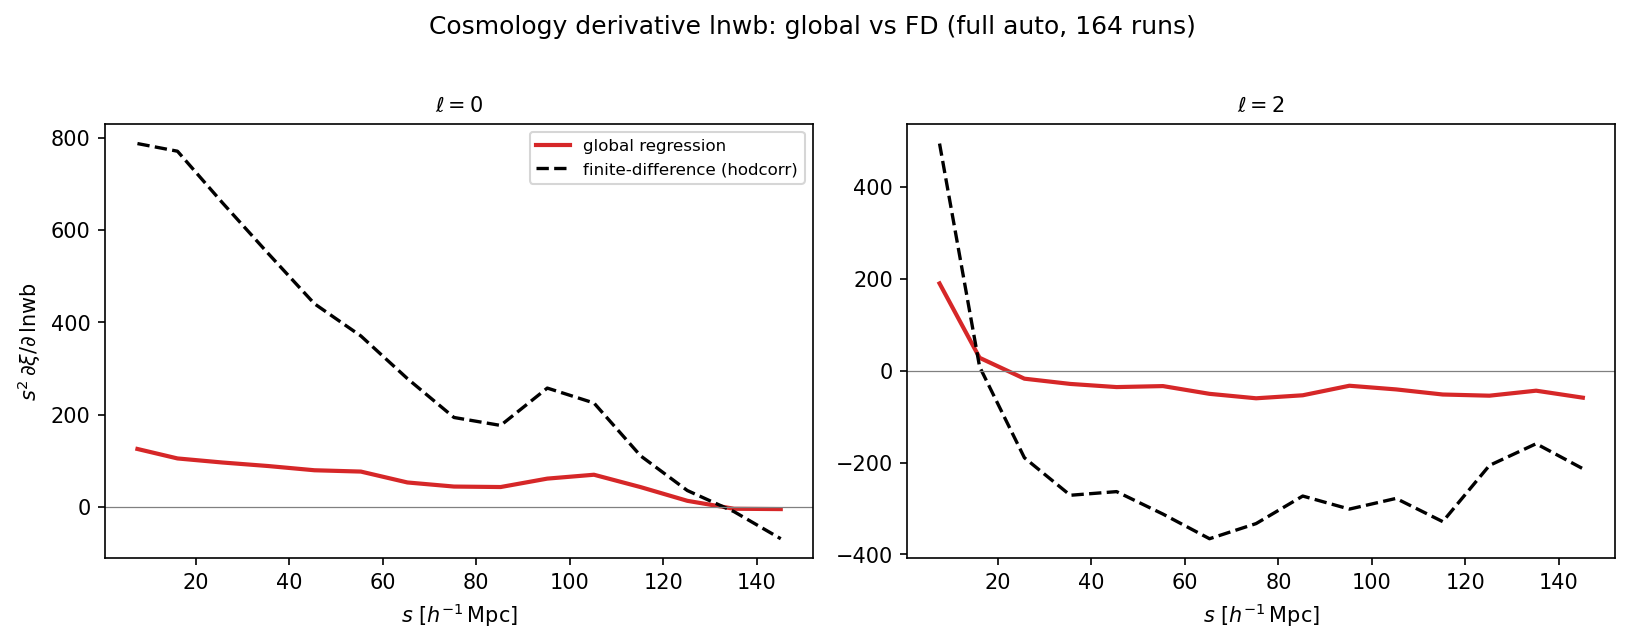
\includegraphics[width=0.49\textwidth]{response_global_vs_fd_lnwb.png}\hfill
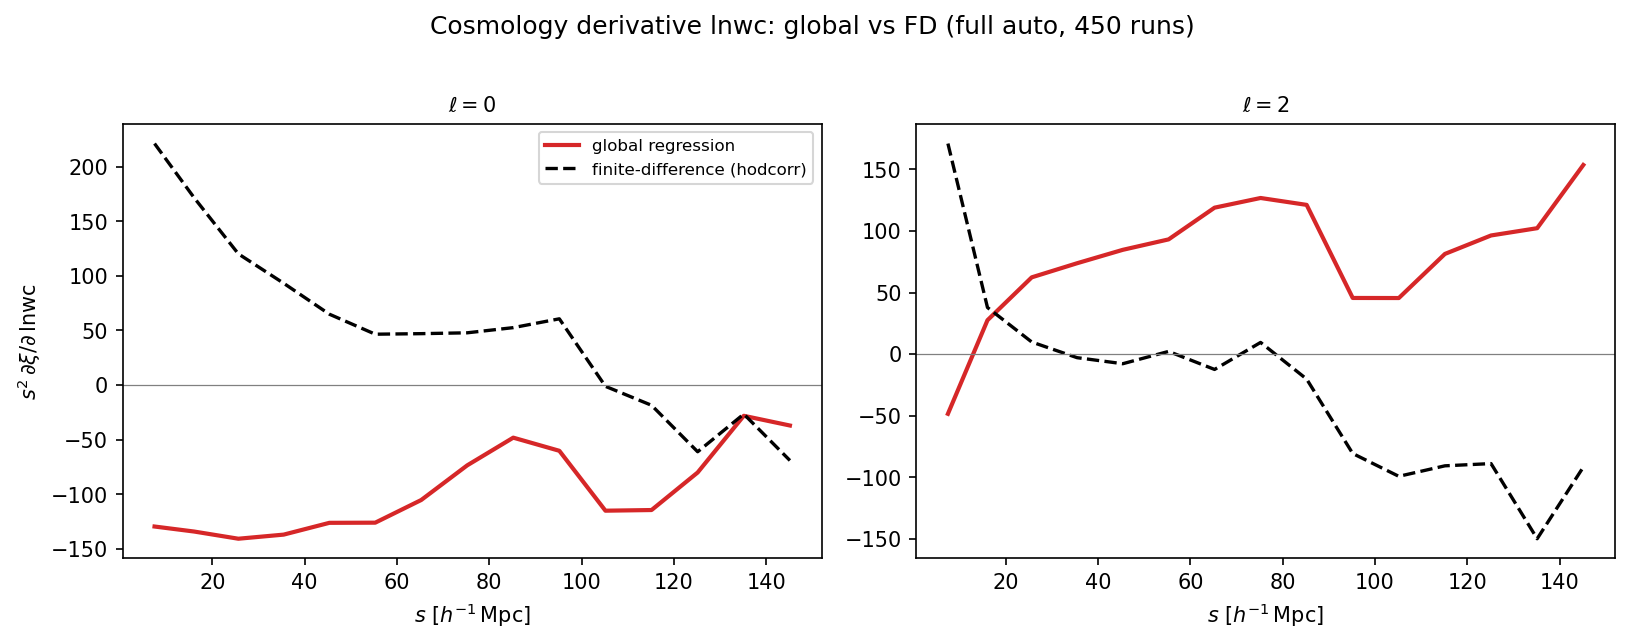
\includegraphics[width=0.49\textwidth]{response_global_vs_fd_lnwc.png}\\[4pt]
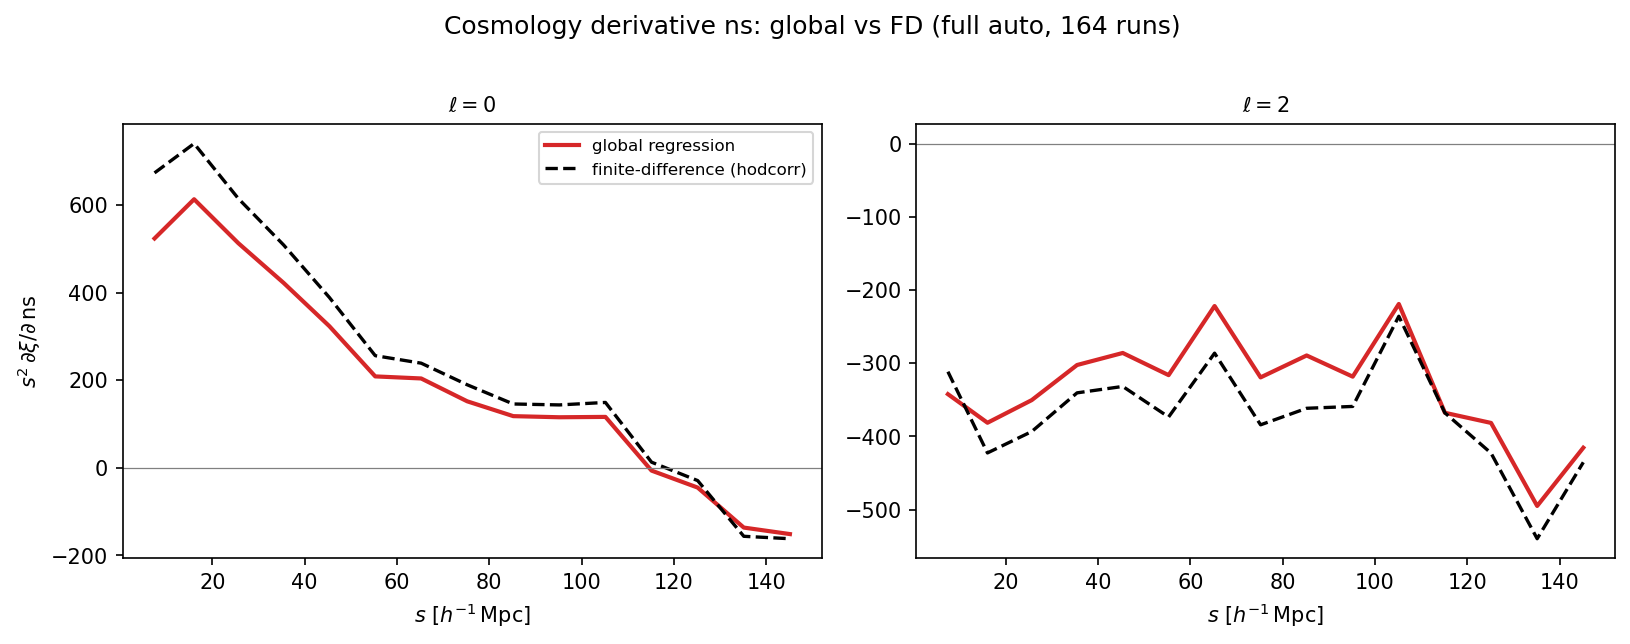
\includegraphics[width=0.49\textwidth]{response_global_vs_fd_ns.png}\hfill
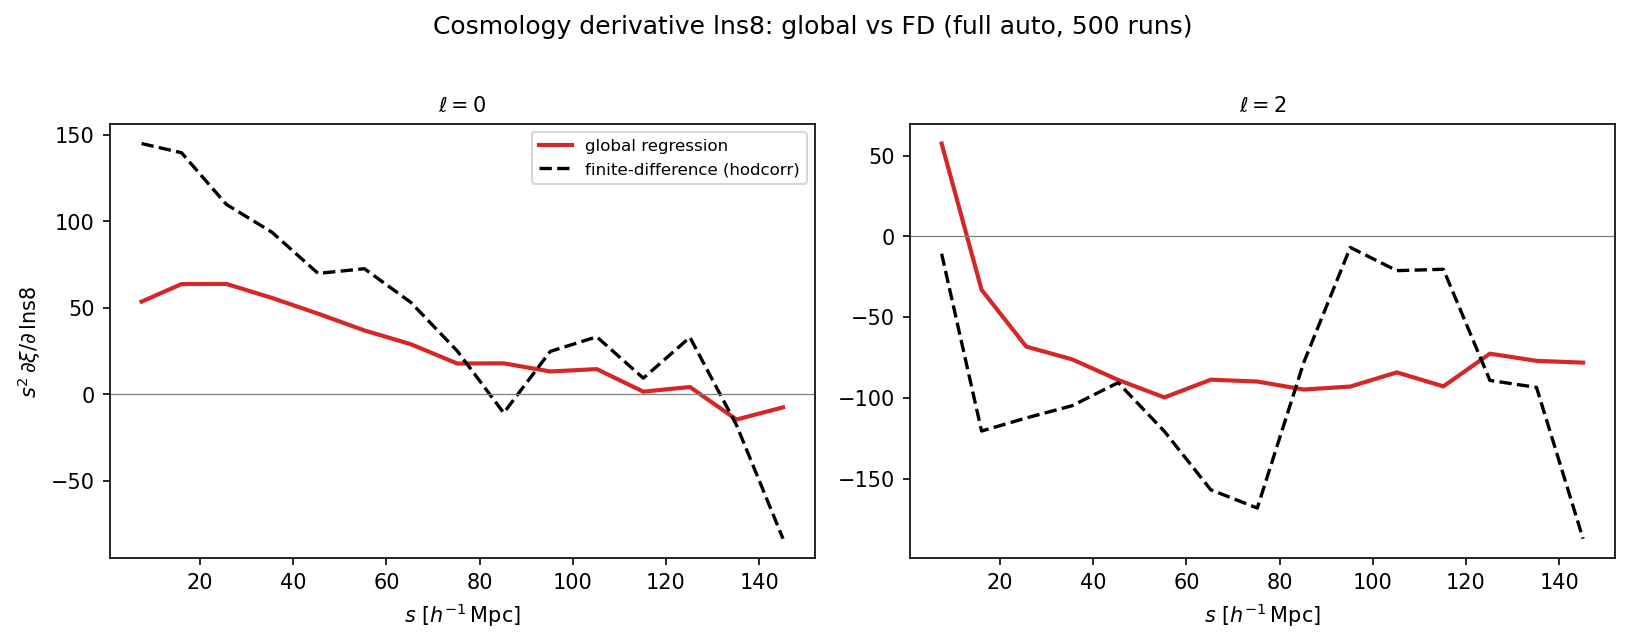
\includegraphics[width=0.49\textwidth]{response_global_vs_fd_lns8.png}
\caption{Cross-check of the global-regression cosmology derivative
(Eq.~\ref{eq:global}, red) against the finite-difference HOD-corrected
derivative (Eq.~\ref{eq:hodcorr}, black dashed) for the full-sample auto,
$\ell=0$ and $\ell=2$.}
\label{fig:globalfd}
\end{figure}

The joint Fisher of Eq.~(\ref{eq:joint}) then consumes the global
derivatives, and we report two marginalisation routes that should agree:
route (a), the $16$-parameter joint Fisher with the yuan23 prior; and route
(b), a prior-free check that adds an empirical HOD covariance
$\mathsf{C}_{\rm HOD}$ --- the sample covariance of the data vector across
the same-phase fiducial HOD ensemble (pure HOD scatter, cosmic variance
cancelled) --- to the cosmic-variance covariance,
$\mathsf{C}_{\rm tot}=\mathsf{C}_{\rm CV}+\mathsf{C}_{\rm HOD}$, and uses
only the 4 cosmology rows.  Table~\ref{tab:global} gives the current
results, spanning data and random quantiles, monopole and quadrupole.

\begin{table}[ht]
\centering
\begin{tabular}{lcccccc}
\toprule
Data vector & $p$ & Hartlap & $\sigma(\omega_b)$ & $\sigma(\omega_{cdm})$ & $\sigma(n_s)$ & $\sigma(\sigma_8)$ \\
\midrule
full auto (mono$+$quad)                 & 30  & 0.95 & $2.12$ & $9.74$ & $52.6$ & $81.5$ \\
data Q autos (mono)                     & 32  & 0.94 & $2.02$ & $7.09$ & $29.5$ & $83.6$ \\
data Q autos (mono$+$quad)              & 64  & 0.89 & $1.45$ & $5.59$ & $17.7$ & $53.9$ \\
rand Q autos (mono$+$quad)              & 64  & 0.89 & $1.35$ & $5.81$ & $21.4$ & $63.4$ \\
data$+$rand Q autos (mono$+$quad)       & 128 & 0.78 & $0.86$ & $3.09$ & $11.2$ & $40.8$ \\
\textbf{full$+$data$+$rand Q autos (mono$+$quad)} & 144 & 0.75 & $\mathbf{0.69}$ & $\mathbf{2.72}$ & $\mathbf{9.76}$ & $\mathbf{36.5}$ \\
\bottomrule
\end{tabular}
\caption{Global-response (route a) HOD-marginalised $\sigma$ (units:
$\omega_b,\omega_{cdm},n_s$ in $10^{-4}$; $\sigma_8$ in $10^{-4}$), pooled
576-sample covariance.  The two marginalisation routes agree to
$1.3$--$1.6\times$ (route b is looser, being prior-free with only 50
$\mathsf{C}_{\rm HOD}$ draws).  These numbers are a smoke test on the 58
runs presently on disk (50 fiducial $+$ 1 per off-fiducial cosmology); the
design-matrix condition number is $1.9$ and $\partial\xi/\partial
\ln\sigma_8$ is $0.68\times 2\xi$, both of which improve as the
$\sim 50$-per-cosmology campaign completes.}
\label{tab:global}
\end{table}

Adding the random quantiles and the quadrupole both help: the random
quantile autos are only slightly weaker than the data quantile autos alone,
but combining data, random, and the full sample with the quadrupole is the
tightest vector on every parameter, because the random quantiles respond to
cosmology and the HOD differently from the galaxies and so break
degeneracies the galaxy clustering alone cannot.

\section{Status and next steps}
\label{sec:status}

The pipeline is complete and the global response model (Eq.~\ref{eq:global})
is the current method.  The $\sim 50$-draw-per-cosmology campaign
($\sim 392$ full-box runs) is in progress; when it finishes, the global
derivatives tighten and the $\partial\xi/\partial\ln\sigma_8 = 2\xi$ sanity
ratio should approach unity.  Remaining limitations are: the covariance
still rests on partially-correlated subboxes (only one phase exists); the
global fit is linear over the HOD prior (a quadratic/interaction extension
would test cosmology-dependence of the HOD response); and derivative-noise
and gradient-uncertainty are not yet propagated into the Fisher.

\begin{thebibliography}{9}

\bibitem{tegmark1997}
M.~Tegmark, A.~N.~Taylor, A.~F.~Heavens,
\emph{Karhunen-Lo\`eve eigenvalue problems in cosmology: how should we
tackle large data sets?}, ApJ 480, 22 (1997).

\bibitem{maksimova2021}
N.~A.~Maksimova et al.,
\emph{AbacusSummit: a massive set of high-accuracy, high-resolution
N-body simulations}, MNRAS 508, 4017 (2021).

\bibitem{hartlap2007}
J.~Hartlap, P.~Simon, P.~Schneider,
\emph{Why your model parameter confidences may be too optimistic.
Unbiased estimation of the inverse covariance matrix},
A\&A 464, 399 (2007).

\end{thebibliography}

\end{document}
